%% 
%% Copyright 2007-2024 Elsevier Ltd
%% 
%% This file is part of the 'Elsarticle Bundle'.
%% ---------------------------------------------
%%  
%% It may be distributed under the conditions of the LaTeX Project Public
%% License, either version 1.3 of this license or (at your option) any%% later version.  The latest version of this license is in
%%    http://www.latex-project.org/lppl.txt
%% and version 1.3 or later is part of all distributions of LaTeX
%% version 1999/12/01 or later.
%% 
%% The list of all files belonging to the 'Elsarticle Bundle' is
 %% given in the file `manifest.txt'.
%% 
%% Template article for Elsevier's document class `elsarticle'
%% with harvard style bibliographic references

\documentclass[preprint,12pt,authoryear]{elsarticle}

%% Use the option review to obtain double line spacing
%% \documentclass[authoryear,preprint,review,12pt]{elsarticle}

%% Use the options 1p,twocolumn; 3p; 3p,twocolumn; 5p; or 5p,twocolumn
%% for a journal layout:
%% \documentclass[final,1p,times,authoryear]{elsarticle}
%% \documentclass[final,1p,times,twocolumn,authoryear]{elsarticle}
%% \documentclass[final,3p,times,authoryear]{elsarticle}
%% \documentclass[final,3p,times,twocolumn,authoryear]{elsarticle}
%% \documentclass[final,5p,times,authoryear]{elsarticle}
%% \documentclass[final,5p,times,twocolumn,authoryear]{elsarticle}

%% For including figures, graphicx.sty has been loaded in
%% elsarticle.cls. If you prefer to use the old commands
%% please give \usepackage{epsfig}

%% The amssymb package provides various useful mathematical symbols
\usepackage{amssymb}
\usepackage{graphicx}
%% The amsmath package provides various useful equation environments.
\usepackage{amsmath}
\usepackage{algorithm}
\usepackage{algorithmicx}
\usepackage{algpseudocode}
%% The amsthm package provides extended theorem environments
%% \usepackage{amsthm}

% Sets
\newcommand{\SetWorkOrder}[1]{W(\VarMetaTime#1)}
\newcommand{\ElementWorkOrder}{w}
\newcommand{\SetPeriod}{P(\VarMetaTime)}
\newcommand{\ElementPeriod}{p}

\newcommand{\SetResource}{R(\VarMetaTime)}
\newcommand{\ElementResource}{r}
\newcommand{\SetOperation}[2]{O_{#1}(\VarMetaTime, #2)}
\newcommand{\ElementOperation}{o}

\newcommand{\SetDays}[1]{D_{#1}(\VarMetaTime)}
\newcommand{\ElementDays}{d}
\newcommand{\SetActivity}[2]{A_{#2}(\VarMetaTime, #1)}
\newcommand{\ElementActivity}{a}

\newcommand{\SetWorkSegment}{K(\VarSupervisorAssignment{}{})}
\newcommand{\ElementWorkSegment}{k}
\newcommand{\SetTimeInstance}{I(\VarMetaTime)}
\newcommand{\ElementTimeInstance}{i}

\newcommand{\SetEvent}{E(\VarMetaTime)}
\newcommand{\ElementEvent}{e}

\newcommand{\SetScheduler}{S}
\newcommand{\ElementScheduler}{s}
\newcommand{\SetSupervisor}{Z}
\newcommand{\ElementSupervisor}{z}

\newcommand{\SetTechnician}{T(\VarMetaTime)}
\newcommand{\ElementTechnician}{t}

% Parameters
\newcommand{\ParStrategicValue}{strategic\_value_{\ElementWorkOrder \ElementPeriod}(\VarMetaTime)}
\newcommand{\ParStrategicPenalty}{strategic\_penalty}
\newcommand{\ParClusteringValue}{clustering\_value_{\ElementWorkOrder1, \ElementWorkOrder2}}
\newcommand{\ParStrategicResource}{resource_{\ElementPeriod\ElementResource}(\VarMetaTime)}

\newcommand{\ParStrategicWorkOrderWeight}{work\_order\_work_{\ElementWorkOrder \ElementResource}}
\newcommand{\ParStrategicInclude}{include(\VarMetaTime)}
\newcommand{\ParStrategicExclude}{exclude(\VarMetaTime)}
\newcommand{\ParTacticalValue}{tactical\_value_{\ElementDays\ElementOperation}(\VarMetaTime)}

\newcommand{\ParTacticalPenalty}{tactical\_penalty}
\newcommand{\ParOperationWork}[1]{work_{#1}(\VarMetaTime)}
\newcommand{\ParTacticalResource}{tactical\_resource_{\ElementDays\ElementResource}(\VarMetaTime)}
\newcommand{\ParStartStart}{start\_start_{\ElementOperation1, \ElementOperation2}}

\newcommand{\ParFinishStart}{finish\_start_{\ElementOperation1, \ElementOperation2}}
\newcommand{\ParEarliestStart}{earliest\_start_{\ElementOperation}(\VarMetaTime)}
\newcommand{\ParLatestFinish}{latest\_finish_{\ElementOperation}(\VarMetaTime)}
\newcommand{\ParNumberOfPeople}{number_{\ElementOperation}(\VarMetaTime)}

\newcommand{\ParOperatingTime}{operating\_time_{\ElementOperation}}
\newcommand{\ParDuration}{duration_{\ElementOperation}(\VarMetaTime)}
\newcommand{\ParSupervisorValue}{supervisor\_value_{\ElementActivity \ElementTechnician}(\VarMetaTime, \VarStartOfSegment{t}{}, \VarFinishOfSegment{t}{})} 
\newcommand{\ParFeasible}{feasible_{at}(\VarIncludeActivity{})}
\newcommand{\ParOperationsForWorkOrder}{work\_order\_to\_operations_{\ElementWorkOrder }}

\newcommand{\ParOperationsInWorkOrder}{operations\_in\_work\_order_{\ElementWorkOrder }}
\newcommand{\ParActivitiesForOperation}{activities\_for\_operation_{\ElementOperation}}
\newcommand{\ParLowerActivityWork}{lower\_activity\_work_{\ElementActivity}(\VarMetaTime)}
\newcommand{\ParActivityWork}[1]{activity\_work_{\ElementActivity}(\VarMetaTime, \VarActivityWork{#1})}

\newcommand{\ParPreparation}{preparation_{\ElementActivity1, \ElementActivity2}}
\newcommand{\ParEvent}{event_{\ElementTimeInstance \ElementEvent}}
\newcommand{\ParEventDuration}{duration_{\ElementTimeInstance \ElementEvent}}
\newcommand{\ParConstraintLimit}{constraint\_limit}

\newcommand{\ParTimeWindowStart}{time\_window\_start_{\ElementActivity}(\VarTacticalWork{}{})}
\newcommand{\ParTimeWindowFinish}{time\_window\_finish_{\ElementActivity}(\VarTacticalWork{}{})}
\newcommand{\ParAvailabilityStart}{availability\_start(\VarMetaTime)}
\newcommand{\ParAvailabilityFinish}{availability\_finish(\VarMetaTime)}

% Variables
\newcommand{\VarStrategicWorkOrderAssignment}[2]{\alpha_{#1#2}(\VarMetaTime)}
\newcommand{\VarStrategicExcess}{\epsilon_{\ElementPeriod\ElementResource}(\VarMetaTime)}
\newcommand{\VarTacticalWork}[2]{\beta_{#1#2}(\VarMetaTime)}
\newcommand{\VarTacticalExcess}{\mu_{\ElementResource \ElementDays}(\VarMetaTime)} 

\newcommand{\VarTacticalWorkBinary}[2]{\sigma_{#1#2}(\VarMetaTime)}
\newcommand{\VarTacticalWorkBinaryConsecutive}{\eta_{\ElementDays\ElementOperation}(\VarMetaTime)}
\newcommand{\VarTacticalOperationDifference}{\Delta_{\ElementOperation}(\VarMetaTime)}
\newcommand{\VarSupervisorAssignment}[2]{\gamma_{#1#2}(\VarMetaTime)}

\newcommand{\VarSupervisorAssignmentWhole}{\phi_{\ElementOperation}(\VarMetaTime)}
\newcommand{\VarActivityWork}[1]{\rho_{#1}(\VarMetaTime)}
\newcommand{\VarProcessingTime}{\delta_{\ElementActivity\ElementWorkSegment}(\VarMetaTime)} 
\newcommand{\VarActiveSegment}[2]{\pi_{#1#2}(\VarMetaTime)}

\newcommand{\VarStartOfSegment}[2]{\lambda_{#1#2}(\VarMetaTime)}
\newcommand{\VarFinishOfSegment}[2]{\Lambda_{#1#2}(\VarMetaTime)}
\newcommand{\VarSegmentInRelation}{\omega_{\ElementActivity\ElementWorkSegment\ElementTimeInstance \ElementEvent}(\VarMetaTime)}
\newcommand{\VarIncludeActivity}[1]{\theta_{#1}(\VarMetaTime)}

% Meta variables
\newcommand{\VarMetaTime}{\tau}


\usepackage[utf8]{inputenc}
\usepackage[T1]{fontenc}
\usepackage{graphicx}
\usepackage{amsmath}
\usepackage{amssymb}
\usepackage{multicol}
\usepackage{natbib}
\usepackage{hyperref}
\usepackage{booktabs} % For professional quality tables
\usepackage{array}    % For better column alignment
%% The lineno packages adds line numbers. Start line numbering with
%% \begin{linenumbers}, end it with \end{linenumbers}. Or switch it on
%% for the whole article with \linenumbers.
%% \usepackage{lineno}

\journal{Computers and Operation Research}

\begin{document}

\begin{frontmatter}

%% Title, authors and addresses

%% use the tnoteref command within \title for footnotes;
%% use the tnotetext command for theassociated footnote;
%% use the fnref command within \author or \affiliation for footnotes;
%% use the fntext command for theassociated footnote;
%% use the corref command within \author for corresponding author footnotes;
%% use the cortext command for theassociated footnote;
%% use the ead command for the email address,
%% and the form \ead[url] for the home page:
%% \title{Title\tnoteref{label1}}
%% \tnotetext[label1]{}
%% \author{Name\corref{cor1}\fnref{label2}}
%% \ead{email address}
%% \ead[url]{home page}
%% \fntext[label2]{}
%% \cortext[cor1]{}
%% \affiliation{organization={},
%%            addressline={}, 
%%            city={},
%%            postcode={}, 
%%            state={},
%%            country={}}
%% \fntext[label3]{}

\title{Actor-based Large Neighborhood Search for weekly maintenance scheduling} %% Article title

%% use optional labels to link authors explicitly to addresses:
%% \author[label1,label2]{}
%% \affiliation[label1]{organization={},
%%             addressline={},
%%             city={},
%%             postcode={},
%%             state={},
%%             country={}}
%%
%% \affiliation[label2]{organization={},
%%             addressline={},
%%             city={},
%%             postcode={},
%%             state={},
%%             country={}}

\author[DTUconstruct]{Christian Brunbjerg Jespersen} %% Author name
\author[DTUconstruct]{Kristoffer Sigsgaard Wernblad}
\author[DTUmanagement]{Thomas Jacob Riis Stidsen}
\author[DTUconstruct]{Kasper Barslund Hansen}
\author[DTUconstruct]{Jingrui Ge}
\author[DTUconstruct]{Simon Didriksen}
\author[DTUconstruct]{Niels Henrik Mortensen}

%% Author affiliation
\affiliation[DTUconstruct]{organization={DTU Construct, Technical University of Denmark},%Department and Organization
            addressline={Anker Egelundsvej 1}, 
            city={Kongens Lyngby},
            postcode={2800}, 
            state={Hovedstaden},
            country={Denmark}}
\affiliation[DTUmanagement]{organization={DTU Management, Technical University of Denmark},%Department and Organization
            addressline={Anker Egelundsvej 1}, 
            city={Kongens Lyngby},
            postcode={2800}, 
            state={Hovedstaden},
            country={Denmark}}
%\affiliation{organization={Technical University of Denmark},%Department and Organization
%            addressline={Anker Egelundsvej 1}, 
%            city={Kongens Lyngby},
%            postcode={2800}, 
%            state={Hovedstaden},
%            country={Denmark}}
%\affiliation{organization={Technical University of Denmark},%Department and Organization
%            addressline={Anker Egelundsvej 1}, 
%            city={Kongens Lyngby},
%            postcode={2800}, 
%            state={Hovedstaden},
%            country={Denmark}}
%\affiliation{organization={Technical University of Denmark},%Department and Organization
%            addressline={Anker Egelundsvej 1}, 
%            city={Kongens Lyngby},
%            postcode={2800}, 
%            state={Hovedstaden},
%            country={Denmark}}
%\affiliation{organization={Technical University of Denmark},%Department and Organization
%            addressline={Anker Egelundsvej 1}, 
%            city={Kongens Lyngby},
%            postcode={2800}, 
%            state={Hovedstaden},
%            country={Denmark}}
%\affiliation{organization={Technical University of Denmark},%Department and Organization
%            addressline={Anker Egelundsvej 1}, 
%            city={Kongens Lyngby},
%            postcode={2800}, 
%            state={Hovedstaden},
%            country={Denmark}}


%% Abstract
\begin{abstract}
%% Text of abstract
Many planning problems facing the operations research field have proven difficult to solve due to their inherent uncertainty and highly dynamic nature. Stochastic Programming~\citep{birge2011introduction}, fuzzy logic~\citep{zadeh1988fuzzy}, and robust optimization~\citep{ben2009robust} are some of the methods that have been proposed to solve these issues. These methods make an implicit assumption of a static data setting and a static problem setting. Maintenance scheduling is one such problem where the best available information continually updates and then therefore the scheduling continuously needs to be updated. Maintenance scheduling is a complex process often more associated with operation management, but here we will argue that is possible to implement general maintenance scheduling approaches, if the solution approach is designed to be integrated into a business
process of the kind that are usually developed by the principles of operation management. 

This paper proposes a novel optimization method that is capable to optimizing a scheduling problem in the following setting:  Primary data source is changing in real-time; external inputs affects the optimization process; multiple actors are making interdependent decision whose objectives may differ significantly. The proposed solution approach is an actor-based framework including a large neighborhood search metaheuristic implementation. The framework is tested on the real-world problem of maintaining scheduling of oil platforms for Total in the North Sea, but the approach is very general and can be applied to a wide variety of other planning problems.
\end{abstract}

%%Graphical abstract
%\begin{graphicalabstract}
%\includegraphics{grabs}
%\end{graphicalabstract}

%%Research highlights
%\begin{highlights}
%\item How to allow direct and real-time integration into an optimization process?
%\item How to perform optimization in a real-time changing parameter space?
%\end{highlights}

%% Keywords
\begin{keyword}
%% keywords here, in the form: keyword \sep keyword
Large Neighborhood Search \sep Actor Framework \sep Maintenance scheduling \sep Real-time Optimization \sep Human-centered Computing \sep Interactive Systems and Tools \sep Decision Support Systems \sep Interactive Optimization.


%% PACS codes here, in the form: \PACS code \sep code

%% MSC codes here, in the form: \MSC code \sep code
%% or \MSC[2008] code \sep code (2000 is the default)

\end{keyword}

\end{frontmatter}

%% Add \usepackage{lineno} before \begin{document} and uncomment 
%% following line to enable line numbers
%% \linenumbers

%% main text
%%

%% Use \section commands to start a section
\section{Introduction}
\label{sec:1-introduction}
%% Labels are used to cross-reference an item using \ref command.

Maintenance scheduling is an operational problem that have proven hard to solve (NP-hard~\citep{garey1979computers}). Furthermore, for optimization to be utilized the dynamic and uncertain nature of maintenance scheduling requires a tight integration with third party administration software to enable the tacit knowledge of decision makers to influence the planning process easily. Often a number of different decision makers at different company levels take part in the planning process and in this way the industry usually assigns responsibility for decision-making  to an individual representing only a small part of the complete process. 

These multiple smaller planning processes are often difficult to map to a single mathematical model describing the whole system as elaborated by~\citep{barthelemy2002human}. Solving operation research problems that are operational in nature have additional requirements over conventional static problems: they have to be responsive to changing parameters; able to be assimilated into the decision-makers workflow; allow for integration with dynamic data sources such as databases and RESTapi~\citep{meignan_review_2015}. Operational aspects of operation research, as opposed to higher level strategic and tactical aspects, are characterized by extensive amounts negotiation and feedback on proposed schedules. The lack of integration and responsiveness can lead to schedules that are not directly implemented in practice but instead provides initial suggestions~\citep{meignan_review_2015}, which are then iterated else where in the scheduling process. In~\citep{barthelemy2002human} the authors argue that many problems that operation research aim to solve are often composed of a group of individuals whose decisions are consolidated into an "epistemic subject" for which a mathematical model can be formulated and solved, with many scheduling problems being good examples. However often multiple actors have different views on what constitutes an optimal schedule hence resulting in multiple-objectives. Even if multi-objective optimization~\citep{ehrgott2002multiple} is applied to find the Pareto Front~\citep{Pareto1897} a negotiating process still is needed between the actors to select the final schedule.

This paper proposes a solution method that will allow for real-time optimization based on actor/user interaction and connection to a dynamic data source, effectively managing the changes to the parameter space. The proposed solution method will be tested on the multi-compartment multi-knapsack problem (MCMKP) for maintenance scheduling on a large dataset from a company. The MCMKP naturally models what in the practical maintenance is called the weekly schedule, taken form \citep{palmerMaintenancePlanningScheduling2019}. It should be noted that the scientific maintenance scheduling literature deviates significantly from its practical implementation which is detailed in \citep{palmerMaintenancePlanningScheduling2019}. The solution method will by based on the large neighborhood search (LNS) metaheuristic. This meta heuristic was chosen due to its properties of naturally being able to work with and fix infeasible solutions and its state of the art performance on various scheduling problems. 

To understand the need for actor-based methods some background knowledge will be required about the maintenance scheduling process. In figure \ref{fig:simple-maintenance-process} illustrates the general setup of a healthy maintenance planning and scheduling system. The systems actors have the following responsibilities: the planner generates the work orders that are to be scheduled; the scheduler creates weekly schedules based on a knapsack formulation; based on the weekly schedule the supervisor assigns work order activities that the work order is composed of (the assignment problem); the technicians executes the work in sequential pattern (single machine scheduling). A final point on the necessity of actor-based approaches to model should a setup is the idea of ownership of a work order. Throughout the scheduling process a work order is owned by a specific actor and he alone is allow to modify it. This means that a single model approach is very difficult to implement in practice as a work order looks different depending on the actor that currently owns it. This also highlight another an point in maintenance scheduling: that the stochastic nature of the maintenance scheduling process can be handled using a change of model each with different levels of aggregation, opposed to more academic approaches such as fuzzy logic and stochastic optimization.

When the fundamental uncertainties manifest themselves during planning or execution work orders are rescheduled by moving between the different actor (models), meaning that the stochastic elements of maintenance scheduling are handled by dynamic rescheduling between the actors.

\begin{figure}

\includegraphics[width=1.0\textwidth]{figures/Scheduling Process Simple.png}
\caption{Simple overview of the scheduling process with its primary types of actors. The planner, the scheduler, the supervisor(s), and the technicians. The green color highlights the scheduler as it the actor in the maintenance scheduling process that is the foundation for the paper.}
\label{fig:simple-maintenance-process}
\end{figure}

This article describes a number of contributions: 

\begin{itemize}
\item A novel actor/optimization framework
\item A novel specialized (A)LNS metaheuristic, to be utilized in an actor framework
\item Implementation and test on a large realworld maintenance scheduling problem
\end{itemize}

The paper is divided into four different sections. Section \ref{sec:2-solution-method} explains the weekly maintenance scheduling model in detail and forms the fundation of the paper. Section \ref{sec:3-results} shows that results coming from the implemented system where the implementation will be affected by simulated user-interaction. Section \ref{sec:4-discussion} will discuss the implications of the research and possible future research directions.

\subsection{A generic maintenance scheduling model}
\label{sub2sec2}
A large company needs to create a weekly maintenance plan for the next $p \in P$ weeks. The maintenance plan is planned centrally and consists of scheduling the $w \in W$ work orders, i.e. maintenance tasks, such that all are scheduled into different weeks. Each work order requires some resourses to be carried out, e.g. man-power with different qualifications, equipment etc. all of these resourses are available in limited amounts and are called traits $\tau \in T$. To simplify matters, we will assume that the recourse limits are not hard but extra workers can be paid overtime, extra equipment can be rented etc., at the cost (penalty) of $pen_{p\tau}$. The urgency of the different maintenance operations varies and is reflected in a penalty for carrying out a maintenance work order in a certain week $v_{wp}(t)$. Urgent tasks have quickly increasing penalties for the later weeks week $p$. Furthermore, two sets exists which will either will require the work order to be carried out in week $p$, i.e. $(w,p) \in E$ and a set which forbids a work order to carried out in week $p$, i.e. $(w,p) \in I$. The model for the problem is the Multi-compartment Multi-knapsack Problem with capacity penalties MCMKP.

The notation used in the model is based on the notation from the dynamic metaheuristics literature as found in \cite{yangMetaheuristicsDynamicCombinatorial2013}, where $t$ is added as a time variable on all sets, parameters, and variables that are subject to change.
This allows us to be precise in the timing on the messages that are send to the Ab-LNS.  

%\subsection{The Weekly Schedule: Multi-compartment Multi-knapsack Problem with capacity penalties}
%\label{sub2sec2}
%The actor-based large neighborhood search is implemented on the MCMKP which models that weekly schedule in maintenance. The model is comprised of five different sets. $P$ is the number of weekly periods; $W$ is the number of work orders; $\tau$ is the number of different traits; $E$ is a set that defines which work orders should be excluded from a specific weekly period; $I$ is an inclusion set that defines the allocation of specific work orders which should be included in a specific weekly period. The model has four parameters. $v_{pw}$ is the value of work order $w$ in weekly period $p$; $d$ is the penalty for exceeding a specific trait capacity; $c_{w\tau}$ is the capacity requirement for work order $w$ for trait $t$; $cap_{p\tau}$ is the total amount of capacity available in for weekly period p for for trait t. The model has 2 decision variables. $x_{wp}$, is a binary decision variable equal to one if work order w is in weekly period p and zero otherwise; $pen_{p\tau}$ is non-negative decision variable equal to the amount of excess capacity above the $cap_{p\tau}$ in weekly period p for trait $\tau$. The parameters $v$, $cap$, $Q$, and $P$ are functions of time, $\tau$, in this case as they will be subject to change during the solution process.


\newpage
\begin{alignat}{2}
	& \text{\rule{\linewidth}{0.4pt}} \notag\\
	& \textbf{Meta variables:} \notag\\
	& \ElementScheduler \in \SetScheduler \\
	& \VarTacticalWork{}{} \\ 
	& \tau \in [0, \infty] \\
	& \text{\rule{\linewidth}{0.4pt}} \notag\\
	& \textbf{Minimize:} \notag                                                                                                                                                        \\
	& \sum_{\ElementWorkOrder \in \SetWorkOrder{}} \sum_{\ElementPeriod \in \SetPeriod} \ParStrategicValue \cdot \VarStrategicWorkOrderAssignment{\ElementWorkOrder}{\ElementPeriod}  \notag\\ 
	& + \sum_{\ElementPeriod \in \SetPeriod} \sum_{\ElementResource \in \SetResource} \ParStrategicPenalty \cdot \VarStrategicExcess     \notag                                              \\
	& + \sum_{\ElementPeriod \in \SetPeriod} \sum_{\ElementWorkOrder1 \in \SetWorkOrder{}} \sum_{\ElementWorkOrder2 \in \SetWorkOrder{}} 	 \quad \ParClusteringValue \cdot \VarStrategicWorkOrderAssignment{\ElementWorkOrder1}{\ElementPeriod} \cdot \VarStrategicWorkOrderAssignment{\ElementWorkOrder2}{\ElementPeriod}  \\
	& \text{\rule{\linewidth}{0.4pt}} \notag\\
	& \textbf{Subject to:} \notag                                                                                                                                                      \\
	& \sum_{\ElementWorkOrder \in \SetWorkOrder{}} \ParStrategicWorkOrderWeight \cdot \VarStrategicWorkOrderAssignment{\ElementWorkOrder}{\ElementPeriod} \leq \ \ParStrategicResource + \VarStrategicExcess                                                                           \quad \forall \ElementPeriod \in \SetPeriod \quad \forall \ElementResource \in \SetResource                                                                                      \\
	& \sum_{\ElementWorkOrder \in \SetWorkOrder{}} \VarStrategicWorkOrderAssignment{\ElementWorkOrder}{\ElementPeriod} = 1              \quad \forall \ElementPeriod \in \SetPeriod                                                                                                                                      \\
	& \VarStrategicWorkOrderAssignment{\ElementWorkOrder}{\ElementPeriod} = 0                                                            \quad \forall (\ElementWorkOrder, \ElementPeriod) \in \ParStrategicExclude                                                                                                       \\
	& \VarStrategicWorkOrderAssignment{\ElementWorkOrder}{\ElementPeriod} = 1                                                            \quad \forall (\ElementWorkOrder, \ElementPeriod) \in \ParStrategicInclude                                                                                                       \\
	& \VarStrategicWorkOrderAssignment{\ElementWorkOrder}{\ElementPeriod} \in \{0, 1\}                                                   \quad \forall \ElementWorkOrder \in \SetWorkOrder{} \quad \forall \ElementPeriod \in \SetPeriod                                                                                 \\ 
	& \VarStrategicExcess \in \mathbb{R}^{+}                                                                                             \quad \forall \ElementPeriod \in \SetPeriod \quad \forall \ElementResource \in \SetResource                                                                                  \\ 
	& \text{\rule{\linewidth}{0.4pt}} \notag
\end{alignat}
\newpage


% \begin{alignat}{2}
% 	& \text{Min} \quad \sum_{w = 1}^{W} \sum_{p = 1}^{P} v_{wp}(t) \cdot x_{wp}(t) + \sum_{p = 1}^{P} \sum_{\tau = 1}^T d \cdot pen_{p\tau}(t)   \label{eqn:objective_function_strategic} \\[1em]
%     & \text{subject to:} \notag                                                                                                                                        \\[1em]
% 	& \sum_{w = 1}^W c_{w\tau} \cdot x_{wp}(t) \leq \ cap_{p\tau}(t) + pen_{p\tau}(t)        && \forall p \in P, \forall \tau \in T                      \label{eqn:capacity_constraint}          \\[1em]
% 	& \sum_{w = 1}^{W} x_{wp}(t) = 1                                            && \forall p \in P                                       \label{eqn:single_workorder_constraint}  \\[1em]
% 	& x_{wp}(t) = 0                                                             && \forall (w, p) \in E(t)                               \label{eqn:exclusion_constraint}         \\[1em]
% 	& x_{wp}(t) = 1                                                             && \forall (w, p) \in I(t)                               \label{eqn:inclusion_constraint}         \\[1em]
% 	& x_{wp}(t) \in \{0, 1\}                                                    && \forall w \in W, \forall p \in P                      \label{eqn:x_integrality_constraint}     \\[1em] 
% 	& pen_{p\tau}(t) \in \mathbb{R}^{+}                                         && \forall p \in P, \forall \tau \in T                      \label{eqn:p_non_negativity_constraint}
% \end{alignat}

The objective function \eqref{eqn:objective_function_strategic_value}, \eqref{eqn:objective_function_strategic_penalty}, and
\eqref{eqn:objective_function_strategic_clustering}
minimizes the total weighted delay of all work order assignments together
with the penalty $\ParStrategicPenalty$ for exceeding the resource capacity given in constraint
\eqref{eqn:capacity_constraint}. The thrid term  
of the model contains the $\ParClusteringValue$ which turns the model into a 
quadratic problem. This term optimizes the value of putting two work orders
in the same period, if they have share similarity like close proximity, 
same functional location, etc. 

Constraint \eqref{eqn:capacity_constraint}
ensures that all the weights $\ParOperationWork{wr}$ for each activity in an work
order, given that it has been assigned, is lower than the capacity for each
period and for each trait $\tau$. $pen_{p\tau}$ is the amount of exceeded
capacity that is needed for the current assignment of work order to be
feasible. Constraint \eqref{eqn:single_workorder_constraint} makes sure
that each work order is assigned to at least a single period. Constraint
\eqref{eqn:exclusion_constraint} excludes a work order from a certain period
and constraint \eqref{eqn:inclusion_constraint} forces a specific work order
to be in a specific period. Constraint \eqref{eqn:x_integrality_constraint} and
\eqref{eqn:p_non_negativity_constraint} specify the variable domain for $x_{wp}$
and $pen_{p\tau}$ respectively. The effects of changing $E$, $I$, $cap$, and $v$
in real-time will be examined to determine their effects on the weekly schedules
and objective value.

% \begin{alignat}{4}   
% \texttt{Min}& 
%  \sum_{\ElementWorkOrder \in \SetWorkOrder{}} \sum_{\ElementPeriod \in \SetPeriod} \ParStrategicValue \cdot \VarStrategicWorkOrderAssignment{\ElementWorkOrder}{\ElementPeriod} \notag \\
%  & + \sum_{\ElementPeriod \in \SetPeriod} \sum_{\ElementResource \in \SetResource} \ParStrategicPenalty \cdot \VarStrategicExcess \notag \\
%  & + \sum_{\ElementPeriod \in \SetPeriod} \sum_{\ElementWorkOrder1 \in \SetWorkOrder{}} \sum_{\ElementWorkOrder2 \in \SetWorkOrder{}} \notag \\
%  & \quad \ParClusteringValue \cdot \VarStrategicWorkOrderAssignment{\ElementWorkOrder1}{\ElementPeriod} \cdot \VarStrategicWorkOrderAssignment{\ElementWorkOrder2}{\ElementPeriod}   
%  % \label{eqn:objective_function_strategic} \\
%  %\quad \sum_{l \in L} \sum_{m \in M} v_{l,m} 
%  %&  \label{mod3:o1}\\
%  \text{s.t.}	\notag\\
%  				& \sum_{i \in I} C^{1}_i \cdot x^k_i & = z^k_1 - z^1_1 & \forall k \in K \label{mod3:setz1}\\
% %& \sum_{\ElementWorkOrder \in \SetWorkOrder{}} \ParStrategicWorkOrderWeight \cdot \VarStrategicWorkOrderAssignment{\ElementWorkOrder}{\ElementPeriod} \notag      \\
%  %&				& \sum_{i \in I} C^{2}_i \cdot x^k_i %& = z^k_2 - z^K_2 & \forall k \in K %\label{mod3:setz2}\\
%  %&				& \sum_{i \in I} w_i \cdot x^k_i %&\leq W & \forall \ \forall k \in %K\label{mod3:knapsack_cons}\\
%  %&              & z^k_2 & \geq l \cdot y_{k,l,m} & %\forall k \in K, l \in L, m \in M %\label{mod3:KsquareLimL}\\
%  %&              & z^k_1 & \geq m \cdot y_{k,l,m} & %\quad \forall k \in K, l \in L, m \in M %\label{mod3:KsquareLimM}\\
%  %&              & \sum_{k \in K} y_{k,l,m} & \geq %v_{l,m} & \forall l \in L, m \in M %\label{mod3:VsquareLimL}\\
%  %&              & x^1_i & = x^{UL}_i & \forall i\in %I \label{mod3:fixUL}\\
%  %&              & x^{K}_i & = x^{LR}_i & \forall %i\in I \label{mod3:fixLR}\\
%  %%&              & v_{l,m} & \leq 0 & \forall l \in %L, m \in M | l \leq z^1_1 \label{mod3:limitREF1}\\
%  %%&              & v_{l,m} & \leq 0 & \forall l \in %L, m \in M | l \leq z^K_2 \label{mod3:limitREF2}\\
%  &				& x_i \in \{0,1\},&z_1,z_2 \in Z+& v_{l,m},y_{k,l,m} \in \{0,1\} \label{mod3:domain}
% \end{alignat}


The objective function \eqref{eqn:objective_function_strategic} minimizes the total weight of all work order assignments together with the penalty $d$ for exceeding the capacity given in constraint \eqref{eqn:capacity_constraint}. Constraint \eqref{eqn:capacity_constraint} ensures that all the weights $c_{w\tau}$ for each activity in an work order, given that it has been assigned, is lower than the capacity for each period and for each trait $\tau$. $pen_{p\tau}$ is the amount of exceeded capacity that is needed for the current assignment of work order to be feasible. Constraint \eqref{eqn:single_workorder_constraint} makes sure that each work order is assigned to at least a single period. Constraint \eqref{eqn:exclusion_constraint} excludes a work order from a certain period and constraint \eqref{eqn:inclusion_constraint} forces a specific work order to be in a specific period. Constraint \eqref{eqn:x_integrality_constraint} and \eqref{eqn:p_non_negativity_constraint} specify the variable domain for $x_{wp}$ and $pen_{p\tau}$ respectively. The effects of changing $E$, $I$, $cap$, and $v$ in real-time will be examined to determine their effects on the weekly schedules and objective value.
\section{Solution Method}
\label{sec:2-solution-method}

\subsection{Actor-based Large Neighborhood Search}
A problem which is affected by user-interaction and requires real-time feedback needs an optimization approach that is able to repair infeasible schedules and while also 
converging quickly. For this the large neighborhood search metaheuristic has been shown satisfy these requirements in the literature \cite{gendreauHandbookMetaheuristics2019}. 

The LNS metaheuristic is defined for static problems, meaning that the parameters that make up the problem instance is not subject to change 
after the algorithm has been started. To make the LNS able adapt to changing parameters in real-time a message system have been implemented into the existing framework. This 
extension is shown in algorithm \ref{algo1}.  

\subsubsection{Messages And Destructors}
LNS in its most basic form has one constructor and one destructor which repeatedly destroy and rebuild the schedule. For the AbLNS we will generalize on this concept by 
including messages as destructors of the classic LNS implementation. This generalization can be seen as being somewhat similar to how the adaptive LNS (ALNS) is formulated,
but where the different constructors and destructors are chosen externally as well. 

Extending on the classic setup we define the following set of destructors, $M$:

\begin{itemize}
	\item $m_1$: Inclusion destruct message	
	\item $m_2$: Exclusion destruct message	
	\item $m_3$: Capacities destruct message	
	\item $m_4$: Weights destruct message	
	\item $m_5$: Random destruct message
\end{itemize}

Each of these messages affect different parts of the MCMK problem (weekly schedule). Notice
here that the first four messages destruct the solution by changing the parameter space and the last message is 
a random destructor.

Generalizing the destructors from being static structures into messages
allows the solution to change in real-time to a changing paramenter space meaning
that the algorithm does not need to restart to handle changes in data. 

\newcommand{\MessageQueue}{Q}
\newcommand{\Solution}{X}
\newcommand{\ProblemInstance}{P}
\newcommand{\SharedSolution}{S}

\begin{algorithm}[H]
\caption{Actor-based Large Neighborhood Search} 
\begin{algorithmic}[1]
\State \textbf{Input} $\MessageQueue$    = message queue
\State \textbf{Input} $\ProblemInstance$ = problem instance
\State \textbf{Input} $\Solution$        = initial schedule
\State \textbf{Input} $\SharedSolution$  = shared solution
% \State $\Solution^b = \Solution$
\Repeat \label{alg:actor-based-large-neighborhood-search:main-optimization-loop}
	\State $\Solution^t = clone(\Solution)$ \label{alg:actor-based-large-neighborhood-search:clone-solution}
	\While{$\MessageQueue.has\_message()$} \label{alg:actor-based-large-neighborhood-search:message-loop}
        % \State $m = queue.pop()$
        % \State $m.destruct(\Solution^b)$
		\State $\ProblemInstance.update(\SharedSolution, m)$
        \State $\Solution^t.destruct(\SharedSolution, m)$
    \EndWhile
	
    \State $\Solution^t.repair(\SharedSolution)$ \label{alg:actor-based-large-neighborhood-search:repair}

    \If{accept($\Solution^t, \Solution$)} \label{alg:actor-based-large-neighborhood-search:accept}                       
        \State $\Solution.update(\Solution^t)$
    \EndIf                                         

    \If{$c(\Solution^t) < c(\Solution)$} \label{alg:actor-based-large-neighborhood-search:better-solution}                             
        \State $\Solution.update(\Solution^t)$
		\State $\SharedSolution.atomic\_pointer\_swap(\Solution)$
    \EndIf                                           
	\State $\MessageQueue.push(m)$ \label{alg:actor-based-large-neighborhood-search:schedule-message}
\Until
\end{algorithmic}
\label{alg:actor-based-large-neighborhood-search}
\end{algorithm}



The basic LNS setup have here been extended with a `message queue`. This message queue will be read from on every iteration of the LNS's main iteration loop. Here we notice that the 
incoming message is able to change both the solution but also the problem instance itself. Here we see one of the defining features of the LNS metaheuristic in play, that due to its inherent property of being able to optimize a solution that have become infeasible which is something that is very likely to happen when you change the parameter of the problem instance itself. 

Another less obvious property the message queue allows is for the algorithm to run indefinitely and instead of restarting the algorithm you instead pass 
messages to it to allow it be adjust both the solution space and the parameter space.
This property avoid the issue of time consuming initial convergence as the algorithm will be found in an optimimal state when the solution is perturbed.

Notice that:

\begin{itemize}
    \item The algorithm responds to changes very quickly, in each iteration (line 5-8. We call this a fine-grained response algorithm
    \item If an improved solution is found, it is immediately being pushed to the data (base). (line 12)
    \item That the optimization occurs in the repair function (line 9), which inserts operations, not scheduled yet in a greedy fashion. While not being an optimal insertion, it is fast
\end{itemize}


\section{Results}\label{sec:3-results}
To test the AbLNS algorithm, several simulations are conducted in which the data
is perturbed during the algorithm’s execution. The data from the
company is presented in Section~\ref{sec:data_instance}. Then the effect of
forcing work orders into specific weekly $\ElementPeriod \in \SetPeriod$
schedules is presented in Section~\ref{sec:response_work_orders} and excluding
work orders from periods is presented in Section~\ref{sec:exclusion}. The
effects of reducing the period resource capacities $\ParStrategicResource$ is
tested in Section~\ref{sec:results:reduced_weekly_capacity} and increasing
$\ElementResource$ is tested in  Section~\ref{sec:increase_week_cap}. Finally
the effect of changing the work order values $\ParStrategicUrgency$, is tested
in Section~\ref{sec:results:strategic_value_changes}.

\subsection{Data Instance}\label{sec:data_instance}
The data instance used in this paper is provided by Total
Energies~\citep{total-energies} and extracted from their SAP ERP system. It
pertains to a specific offshore platform and covers a two-year time horizon. The
instance includes 3,487 outstanding work orders ($\SetWorkOrder{}$), 16 distinct
resource skill sets ($\SetResource$) (e.g., mechanics, electricians, turbine
specialists, etc.), and spans 52 bi-weekly periods ($\SetPeriod$), roughly
equivalent to two years.
 
\begin{table}[H]
\centering
\begin{tabular}{lrrrr}
\toprule
           & $|\SetWorkOrder{}|$ & $|\SetResource|$ & $|\SetPeriod|$ \\ \midrule
Instance 1 & 3487                & 16               & 52             \\ \bottomrule
\end{tabular}

\caption{Specific data instances from the case company. Here $\SetWorkOrder$ is the set of work orders, $\SetResource$ is the set of resources, and $\SetPeriod$ is the set of weekly periods.} % \label{fig1}
\end{table}

\subsection{Value of Objective Function Parameters}
The optimization problem has three terms and it could be argued that the
a pareto front should be calculated on the value of the different weightings
between them. To not lose sight of the main contribution of the paper the
value of the $\ParClusteringValue$ and $\ParStrategicPenalty$ has been set so
that the $\ParStrategicPenalty$ always dominates the $\ParStrategicUrgency$ and
that the $\ParStrategicUrgency$ always dominates the $\ParClusteringValue$.
Furthermore the $\ParClusteringValue$ has been excluded from the results section
to put more focus on the user-input interaction.

\subsection{Response to Inclusion of Work Orders}\label{sec:response_work_orders}
The $\ParStrategicInclude$ parameter specifies whether a work order
should be scheduled into a specific period. As the parameter has the time
variable $\VarMetaTime$ it means that this parameter can change at any time
while the metaheuristic is running. The $\ParStrategicInclude$ parameter
constrains the model in equation~\ref{eqn:constraint:strategic:include}.
Table~\ref{tab:responses:inclusion} shows the responses that the model will be
subject to while it is running for different timepoints $\VarMetaTime$.

\begin{table}[H]
	\centering
	\begin{tabular}{lrrrrr}
	\toprule
	                                & $\VarMetaTime_1 = 60$ & $\VarMetaTime_2 = 120$ & $\VarMetaTime_3 = 180$ & $\VarMetaTime_4 = 240$ & $\VarMetaTime_5 = 300$ \\ \midrule
	$\Delta \ParStrategicInclude$ & 50                    & 50                     & 50                     & 50                     & 50                     \\ \bottomrule
	\end{tabular}
	\caption{The including work orders perturbations that the AbLNS will be affected by. 
		Perturbations occur at 60 second time intervals affecting 50 randomly chosen work orders included into random periods.
	}\label{tab:responses:inclusion}
\end{table}

Figure~\ref{fig:responses:inclusion} shows the effects of changing the $
\ParStrategicInclude$ parameter in real-time. The model quickly converges
and when the system is pertubed by an input response the objective 
value~\ref{eqn:objective:strategic} shows a small spike and then quickly converges to
a new solution.

\begin{figure}[H]
	\centering
	\resizebox{10cm}{!}{
		\tikzpicture[gnuplot]
%% generated with GNUPLOT 6.0p1 (Lua 5.2; terminal rev. Jun 2020, script rev. 118)
%% Mon 06 Jan 2025 03:43:49 PM UTC
\path (0.000,0.000) rectangle (16.000,12.000);
\gpcolor{rgb color={0.753,0.753,0.753}}
\gpsetlinetype{gp lt border}
\gpsetdashtype{gp dt solid}
\gpsetlinewidth{2.00}
\draw[gp path] (2.424,1.845)--(13.667,1.845);
\gpcolor{color=gp lt color border}
\gpsetlinewidth{1.00}
\draw[gp path] (2.424,1.845)--(2.604,1.845);
\node[gp node right] at (2.240,1.845) {$8.85\times10^{10}$};
\gpcolor{rgb color={0.753,0.753,0.753}}
\gpsetlinewidth{2.00}
\draw[gp path] (2.424,3.383)--(13.667,3.383);
\gpcolor{color=gp lt color border}
\gpsetlinewidth{1.00}
\draw[gp path] (2.424,3.383)--(2.604,3.383);
\node[gp node right] at (2.240,3.383) {$8.9\times10^{10}$};
\gpcolor{rgb color={0.753,0.753,0.753}}
\gpsetlinewidth{2.00}
\draw[gp path] (2.424,4.922)--(13.667,4.922);
\gpcolor{color=gp lt color border}
\gpsetlinewidth{1.00}
\draw[gp path] (2.424,4.922)--(2.604,4.922);
\node[gp node right] at (2.240,4.922) {$8.95\times10^{10}$};
\gpcolor{rgb color={0.753,0.753,0.753}}
\gpsetlinewidth{2.00}
\draw[gp path] (2.424,6.460)--(13.667,6.460);
\gpcolor{color=gp lt color border}
\gpsetlinewidth{1.00}
\draw[gp path] (2.424,6.460)--(2.604,6.460);
\node[gp node right] at (2.240,6.460) {$9\times10^{10}$};
\gpcolor{rgb color={0.753,0.753,0.753}}
\gpsetlinewidth{2.00}
\draw[gp path] (2.424,7.998)--(13.667,7.998);
\gpcolor{color=gp lt color border}
\gpsetlinewidth{1.00}
\draw[gp path] (2.424,7.998)--(2.604,7.998);
\node[gp node right] at (2.240,7.998) {$9.05\times10^{10}$};
\gpcolor{rgb color={0.753,0.753,0.753}}
\gpsetlinewidth{2.00}
\draw[gp path] (2.424,9.537)--(7.047,9.537);
\draw[gp path] (13.483,9.537)--(13.667,9.537);
\gpcolor{color=gp lt color border}
\gpsetlinewidth{1.00}
\draw[gp path] (2.424,9.537)--(2.604,9.537);
\node[gp node right] at (2.240,9.537) {$9.1\times10^{10}$};
\gpcolor{rgb color={0.753,0.753,0.753}}
\gpsetlinewidth{2.00}
\draw[gp path] (2.424,11.075)--(13.667,11.075);
\gpcolor{color=gp lt color border}
\gpsetlinewidth{1.00}
\draw[gp path] (2.424,11.075)--(2.604,11.075);
\node[gp node right] at (2.240,11.075) {$9.15\times10^{10}$};
\gpcolor{rgb color={0.753,0.753,0.753}}
\gpsetlinewidth{2.00}
\draw[gp path] (2.424,1.845)--(2.424,11.075);
\gpcolor{color=gp lt color border}
\gpsetlinewidth{1.00}
\draw[gp path] (2.424,1.845)--(2.424,2.025);
\draw[gp path] (2.424,11.075)--(2.424,10.895);
\node[gp node left,rotate=270] at (2.424,1.661) {$0$};
\gpcolor{rgb color={0.753,0.753,0.753}}
\gpsetlinewidth{2.00}
\draw[gp path] (4.030,1.845)--(4.030,11.075);
\gpcolor{color=gp lt color border}
\gpsetlinewidth{1.00}
\draw[gp path] (4.030,1.845)--(4.030,2.025);
\draw[gp path] (4.030,11.075)--(4.030,10.895);
\node[gp node left,rotate=270] at (4.030,1.661) {$50$};
\gpcolor{rgb color={0.753,0.753,0.753}}
\gpsetlinewidth{2.00}
\draw[gp path] (5.636,1.845)--(5.636,11.075);
\gpcolor{color=gp lt color border}
\gpsetlinewidth{1.00}
\draw[gp path] (5.636,1.845)--(5.636,2.025);
\draw[gp path] (5.636,11.075)--(5.636,10.895);
\node[gp node left,rotate=270] at (5.636,1.661) {$100$};
\gpcolor{rgb color={0.753,0.753,0.753}}
\gpsetlinewidth{2.00}
\draw[gp path] (7.242,1.845)--(7.242,9.355);
\draw[gp path] (7.242,10.895)--(7.242,11.075);
\gpcolor{color=gp lt color border}
\gpsetlinewidth{1.00}
\draw[gp path] (7.242,1.845)--(7.242,2.025);
\draw[gp path] (7.242,11.075)--(7.242,10.895);
\node[gp node left,rotate=270] at (7.242,1.661) {$150$};
\gpcolor{rgb color={0.753,0.753,0.753}}
\gpsetlinewidth{2.00}
\draw[gp path] (8.849,1.845)--(8.849,9.355);
\draw[gp path] (8.849,10.895)--(8.849,11.075);
\gpcolor{color=gp lt color border}
\gpsetlinewidth{1.00}
\draw[gp path] (8.849,1.845)--(8.849,2.025);
\draw[gp path] (8.849,11.075)--(8.849,10.895);
\node[gp node left,rotate=270] at (8.849,1.661) {$200$};
\gpcolor{rgb color={0.753,0.753,0.753}}
\gpsetlinewidth{2.00}
\draw[gp path] (10.455,1.845)--(10.455,9.355);
\draw[gp path] (10.455,10.895)--(10.455,11.075);
\gpcolor{color=gp lt color border}
\gpsetlinewidth{1.00}
\draw[gp path] (10.455,1.845)--(10.455,2.025);
\draw[gp path] (10.455,11.075)--(10.455,10.895);
\node[gp node left,rotate=270] at (10.455,1.661) {$250$};
\gpcolor{rgb color={0.753,0.753,0.753}}
\gpsetlinewidth{2.00}
\draw[gp path] (12.061,1.845)--(12.061,9.355);
\draw[gp path] (12.061,10.895)--(12.061,11.075);
\gpcolor{color=gp lt color border}
\gpsetlinewidth{1.00}
\draw[gp path] (12.061,1.845)--(12.061,2.025);
\draw[gp path] (12.061,11.075)--(12.061,10.895);
\node[gp node left,rotate=270] at (12.061,1.661) {$300$};
\gpcolor{rgb color={0.753,0.753,0.753}}
\gpsetlinewidth{2.00}
\draw[gp path] (13.667,1.845)--(13.667,11.075);
\gpcolor{color=gp lt color border}
\gpsetlinewidth{1.00}
\draw[gp path] (13.667,1.845)--(13.667,2.025);
\draw[gp path] (13.667,11.075)--(13.667,10.895);
\node[gp node left,rotate=270] at (13.667,1.661) {$350$};
\draw[gp path] (13.667,1.845)--(13.487,1.845);
\node[gp node left] at (13.851,1.845) {$102000$};
\draw[gp path] (13.667,3.164)--(13.487,3.164);
\node[gp node left] at (13.851,3.164) {$103000$};
\draw[gp path] (13.667,4.482)--(13.487,4.482);
\node[gp node left] at (13.851,4.482) {$104000$};
\draw[gp path] (13.667,5.801)--(13.487,5.801);
\node[gp node left] at (13.851,5.801) {$105000$};
\draw[gp path] (13.667,7.119)--(13.487,7.119);
\node[gp node left] at (13.851,7.119) {$106000$};
\draw[gp path] (13.667,8.438)--(13.487,8.438);
\node[gp node left] at (13.851,8.438) {$107000$};
\draw[gp path] (13.667,9.756)--(13.487,9.756);
\node[gp node left] at (13.851,9.756) {$108000$};
\draw[gp path] (13.667,11.075)--(13.487,11.075);
\node[gp node left] at (13.851,11.075) {$109000$};
\draw[gp path] (2.424,11.075)--(2.424,1.845)--(13.667,1.845)--(13.667,11.075)--cycle;
\draw[gp path] (7.047,9.355)--(7.047,10.895)--(13.483,10.895)--(13.483,9.355)--cycle;
\node[gp node right] at (12.199,10.510) {Strategic urgency};
\gpcolor{rgb color={0.000,0.000,0.000}}
\gpsetlinewidth{2.50}
\draw[gp path] (12.383,10.510)--(13.299,10.510);
\draw[gp path] (2.424,2.222)--(2.424,2.236)--(2.424,2.405)--(2.424,2.338)--(2.424,2.361)%
  --(2.424,2.819)--(2.456,3.178)--(2.456,4.057)--(2.456,4.163)--(2.456,4.366)--(2.456,4.711)%
  --(2.456,4.877)--(2.456,4.986)--(2.456,5.164)--(2.456,5.190)--(2.456,5.376)--(2.456,5.421)%
  --(2.456,5.401)--(2.456,5.692)--(2.456,5.583)--(2.456,5.840)--(2.456,5.824)--(2.456,6.014)%
  --(2.456,6.473)--(2.456,6.903)--(2.456,7.279)--(2.456,7.695)--(2.456,7.539)--(2.456,7.569)%
  --(2.456,8.194)--(2.456,8.416)--(2.456,8.452)--(2.456,8.416)--(2.456,8.510)--(2.456,8.617)%
  --(2.456,8.559)--(2.456,8.355)--(2.456,8.410)--(2.456,8.292)--(2.456,8.382)--(2.456,8.591)%
  --(2.456,8.948)--(2.456,9.087)--(2.456,9.102)--(2.456,8.972)--(2.456,8.877)--(2.456,8.819)%
  --(2.456,8.801)--(2.456,8.728)--(2.456,8.793)--(2.456,8.857)--(2.456,8.971)--(2.456,9.176)%
  --(2.456,9.500)--(2.456,9.614)--(2.456,9.511)--(2.456,9.634)--(2.456,9.595)--(2.456,9.666)%
  --(2.456,9.537)--(2.456,9.606)--(2.456,9.600)--(2.456,9.475)--(2.456,9.544)--(2.456,9.480)%
  --(2.456,9.498)--(2.456,9.477)--(2.456,9.396)--(2.456,9.444)--(2.456,9.451)--(2.456,9.527)%
  --(2.488,9.493)--(2.488,9.325)--(2.488,9.370)--(2.488,9.276)--(2.488,9.016)--(2.488,9.091)%
  --(2.488,9.062)--(2.488,9.143)--(2.488,9.157)--(2.488,9.105)--(2.488,9.003)--(2.488,8.978)%
  --(2.488,9.211)--(2.488,9.190)--(2.488,9.145)--(2.488,9.114)--(2.488,9.092)--(2.488,9.204)%
  --(2.488,9.657)--(2.488,9.543)--(2.488,9.528)--(2.488,9.566)--(2.488,9.680)--(2.488,9.636)%
  --(2.488,9.587)--(2.488,9.583)--(2.488,9.483)--(2.488,9.446)--(2.488,9.495)--(2.520,9.375)%
  --(2.520,9.261)--(2.520,9.174)--(2.520,9.403)--(2.520,9.323)--(2.520,9.283)--(2.520,9.212)%
  --(2.520,9.073)--(2.520,9.031)--(2.520,9.026)--(2.520,9.029)--(2.520,8.932)--(2.520,8.860)%
  --(2.520,8.820)--(2.520,8.769)--(2.520,8.789)--(2.520,8.774)--(2.520,8.905)--(2.520,8.854)%
  --(2.520,8.857)--(2.520,8.853)--(2.520,8.964)--(2.520,9.105)--(2.520,9.018)--(2.520,8.863)%
  --(2.520,8.862)--(2.520,8.851)--(2.520,8.848)--(2.520,8.843)--(2.552,8.774)--(2.552,8.723)%
  --(2.552,8.701)--(2.552,8.628)--(2.552,8.584)--(2.552,8.585)--(2.552,8.568)--(2.552,8.434)%
  --(2.552,8.423)--(2.552,8.334)--(2.552,8.204)--(2.552,8.172)--(2.552,8.134)--(2.552,8.121)%
  --(2.552,8.120)--(2.552,8.091)--(2.585,7.969)--(2.585,7.949)--(2.585,7.945)--(2.585,7.933)%
  --(2.585,7.930)--(2.585,7.912)--(2.585,7.884)--(2.585,7.805)--(2.585,7.755)--(2.585,7.745)%
  --(2.585,7.744)--(2.585,7.732)--(2.585,7.727)--(2.585,7.664)--(2.585,7.625)--(2.585,7.620)%
  --(2.585,7.594)--(2.585,7.571)--(2.585,7.559)--(2.617,7.528)--(2.617,7.515)--(2.617,7.492)%
  --(2.617,7.483)--(2.617,7.453)--(2.617,7.346)--(2.617,7.319)--(2.617,7.305)--(2.617,7.295)%
  --(2.617,7.293)--(2.617,7.288)--(2.649,7.273)--(2.649,7.122)--(2.649,7.098)--(2.649,7.091)%
  --(2.681,7.062)--(2.681,7.060)--(2.681,7.005)--(2.681,6.999)--(2.681,6.962)--(2.681,6.928)%
  --(2.681,6.908)--(2.713,6.904)--(2.713,6.894)--(2.713,6.853)--(2.713,6.815)--(2.713,6.787)%
  --(2.713,6.780)--(2.745,6.766)--(2.745,6.733)--(2.745,6.726)--(2.745,6.706)--(2.777,6.658)%
  --(2.777,6.631)--(2.809,6.631)--(2.809,6.613)--(2.809,6.595)--(2.809,6.573)--(2.809,6.534)%
  --(2.809,6.499)--(2.809,6.491)--(2.809,6.468)--(2.809,6.495)--(2.809,6.484)--(2.809,6.475)%
  --(2.809,6.464)--(2.809,6.448)--(2.842,6.417)--(2.842,6.363)--(2.842,6.357)--(2.874,6.357)%
  --(2.874,6.343)--(2.874,6.329)--(2.874,6.358)--(2.874,6.320)--(2.906,6.313)--(2.906,6.291)%
  --(2.938,6.268)--(2.938,6.176)--(2.938,6.172)--(2.938,6.140)--(2.938,6.138)--(2.970,6.110)%
  --(2.970,6.067)--(3.034,6.029)--(3.066,5.985)--(3.066,5.968)--(3.099,5.934)--(3.099,5.888)%
  --(3.163,5.858)--(3.195,5.848)--(3.195,5.826)--(3.195,5.763)--(3.195,5.749)--(3.195,5.746)%
  --(3.195,5.734)--(3.227,5.728)--(3.259,5.717)--(3.259,5.708)--(3.259,5.686)--(3.259,5.682)%
  --(3.291,5.667)--(3.291,5.645)--(3.356,5.635)--(3.388,5.606)--(3.420,5.606)--(3.420,5.603)%
  --(3.484,5.581)--(3.516,5.561)--(3.516,5.532)--(3.516,5.530)--(3.548,5.507)--(3.548,5.479)%
  --(3.645,5.473)--(3.709,5.469)--(3.709,5.468)--(3.741,5.455)--(3.773,5.449)--(3.837,5.445)%
  --(3.902,5.435)--(3.902,4.747)--(3.902,4.789)--(3.902,4.928)--(3.902,5.022)--(3.902,5.178)%
  --(3.902,5.113)--(3.902,5.257)--(3.902,5.440)--(3.902,5.603)--(3.902,5.950)--(3.902,6.056)%
  --(3.902,6.514)--(3.902,6.540)--(3.902,6.579)--(3.902,6.568)--(3.902,6.485)--(3.902,6.472)%
  --(3.934,6.576)--(3.934,6.567)--(3.934,6.518)--(3.934,6.523)--(3.934,6.628)--(3.934,6.646)%
  --(3.934,6.546)--(3.934,6.806)--(3.934,6.846)--(3.934,6.820)--(3.934,6.903)--(3.934,6.950)%
  --(3.934,6.875)--(3.934,6.716)--(3.934,6.707)--(3.934,6.678)--(3.934,6.643)--(3.966,6.680)%
  --(3.966,6.741)--(3.966,6.736)--(3.966,6.742)--(3.966,6.717)--(3.966,6.683)--(3.966,6.795)%
  --(3.966,6.808)--(3.966,6.744)--(3.966,6.776)--(3.998,6.745)--(3.998,6.717)--(3.998,6.716)%
  --(3.998,6.803)--(3.998,6.772)--(3.998,6.839)--(3.998,6.818)--(4.030,6.788)--(4.030,6.774)%
  --(4.030,6.766)--(4.030,6.723)--(4.062,6.718)--(4.062,6.704)--(4.062,6.661)--(4.062,6.686)%
  --(4.062,6.642)--(4.062,6.602)--(4.062,6.529)--(4.094,6.508)--(4.094,6.477)--(4.094,6.467)%
  --(4.159,6.466)--(4.159,6.450)--(4.191,6.435)--(4.191,6.390)--(4.191,6.360)--(4.191,6.329)%
  --(4.223,6.328)--(4.223,6.304)--(4.223,6.291)--(4.223,6.278)--(4.255,6.263)--(4.287,6.257)%
  --(4.287,6.250)--(4.319,6.239)--(4.351,6.198)--(4.351,6.182)--(4.383,6.155)--(4.383,6.131)%
  --(4.416,6.109)--(4.416,6.098)--(4.480,6.093)--(4.480,6.064)--(4.480,6.089)--(4.480,6.081)%
  --(4.512,6.075)--(4.512,6.064)--(4.544,6.044)--(4.576,6.018)--(4.576,6.014)--(4.576,5.984)%
  --(4.608,5.977)--(4.640,5.918)--(4.640,5.907)--(4.640,5.903)--(4.640,5.874)--(4.640,5.852)%
  --(4.640,5.842)--(4.673,5.826)--(4.769,5.789)--(4.769,5.745)--(4.801,5.744)--(4.801,5.713)%
  --(4.865,5.712)--(4.865,5.711)--(4.897,5.710)--(4.897,5.709)--(4.897,5.704)--(4.897,5.681)%
  --(4.930,5.668)--(4.930,5.667)--(4.962,5.656)--(4.962,5.624)--(4.962,5.599)--(4.962,5.533)%
  --(5.058,5.506)--(5.058,5.505)--(5.122,5.496)--(5.219,5.492)--(5.315,5.447)--(5.636,5.447)%
  --(5.668,5.432)--(5.765,5.394)--(5.797,5.365)--(5.829,5.316)--(5.829,5.281)--(5.829,5.210)%
  --(5.829,5.291)--(5.829,5.280)--(5.829,5.265)--(5.829,5.548)--(5.829,5.588)--(5.829,5.699)%
  --(5.829,5.819)--(5.829,5.742)--(5.829,5.906)--(5.829,5.892)--(5.829,5.994)--(5.829,5.943)%
  --(5.829,5.932)--(5.861,6.049)--(5.861,6.010)--(5.861,6.021)--(5.861,6.018)--(5.861,5.986)%
  --(5.861,6.064)--(5.861,6.044)--(5.861,6.309)--(5.861,6.499)--(5.861,6.533)--(5.861,6.550)%
  --(5.861,6.662)--(5.861,6.614)--(5.861,6.592)--(5.861,6.547)--(5.861,6.593)--(5.861,6.571)%
  --(5.861,6.564)--(5.861,6.539)--(5.861,6.521)--(5.893,6.511)--(5.893,6.507)--(5.893,6.477)%
  --(5.893,6.462)--(5.893,6.631)--(5.893,6.528)--(5.893,6.504)--(5.893,6.485)--(5.893,6.484)%
  --(5.893,6.519)--(5.893,6.518)--(5.893,6.509)--(5.893,6.446)--(5.893,6.405)--(5.893,6.404)%
  --(5.893,6.388)--(5.925,6.291)--(5.958,6.270)--(5.958,6.183)--(5.958,6.164)--(5.958,6.270)%
  --(5.990,6.226)--(5.990,6.207)--(5.990,6.161)--(5.990,6.157)--(5.990,6.136)--(6.022,6.077)%
  --(6.022,6.056)--(6.022,6.053)--(6.022,6.017)--(6.022,5.920)--(6.054,5.946)--(6.054,5.925)%
  --(6.054,5.888)--(6.054,5.861)--(6.054,5.931)--(6.054,5.888)--(6.054,5.856)--(6.086,5.846)%
  --(6.086,5.805)--(6.086,5.766)--(6.086,5.743)--(6.086,5.709)--(6.118,5.698)--(6.118,5.690)%
  --(6.118,5.667)--(6.118,5.646)--(6.150,5.645)--(6.182,5.601)--(6.182,5.582)--(6.182,5.567)%
  --(6.214,5.565)--(6.214,5.563)--(6.214,5.552)--(6.214,5.519)--(6.214,5.516)--(6.247,5.515)%
  --(6.247,5.509)--(6.247,5.491)--(6.279,5.485)--(6.311,5.472)--(6.311,5.445)--(6.343,5.423)%
  --(6.343,5.421)--(6.343,5.410)--(6.375,5.397)--(6.375,5.334)--(6.375,5.330)--(6.375,5.326)%
  --(6.375,5.271)--(6.407,5.259)--(6.407,5.257)--(6.407,5.252)--(6.407,5.239)--(6.439,5.213)%
  --(6.439,5.207)--(6.439,5.162)--(6.439,5.183)--(6.471,5.145)--(6.471,5.133)--(6.504,5.118)%
  --(6.504,5.117)--(6.536,5.109)--(6.536,5.106)--(6.664,5.106)--(6.664,5.104)--(6.728,5.102)%
  --(6.793,5.096)--(6.825,5.093)--(6.825,5.090)--(6.889,5.075)--(6.921,5.071)--(6.921,5.053)%
  --(6.985,5.053)--(7.018,5.026)--(7.050,5.019)--(7.050,5.018)--(7.146,5.012)--(7.178,4.989)%
  --(7.210,4.953)--(7.275,4.936)--(7.371,4.924)--(7.371,4.921)--(7.403,4.914)--(7.403,4.911)%
  --(7.403,4.902)--(7.564,4.891)--(7.564,4.865)--(7.596,4.861)--(7.596,4.858)--(7.660,4.836)%
  --(7.660,4.831)--(7.692,4.829)--(7.724,4.826)--(7.756,5.302)--(7.756,5.443)--(7.756,5.694)%
  --(7.756,5.838)--(7.756,5.774)--(7.756,5.689)--(7.756,5.656)--(7.756,5.782)--(7.756,5.779)%
  --(7.756,5.918)--(7.756,6.019)--(7.756,5.982)--(7.789,5.923)--(7.789,5.880)--(7.789,6.043)%
  --(7.789,6.033)--(7.789,6.022)--(7.789,6.178)--(7.789,6.147)--(7.789,6.382)--(7.789,6.468)%
  --(7.789,6.674)--(7.789,6.591)--(7.789,6.615)--(7.789,6.691)--(7.789,6.715)--(7.789,6.700)%
  --(7.789,6.668)--(7.789,6.643)--(7.789,6.867)--(7.789,6.816)--(7.789,6.787)--(7.789,6.792)%
  --(7.789,6.813)--(7.789,6.786)--(7.789,6.836)--(7.789,6.840)--(7.789,6.789)--(7.821,6.785)%
  --(7.821,6.706)--(7.821,6.688)--(7.821,6.667)--(7.821,6.648)--(7.821,6.619)--(7.853,6.588)%
  --(7.853,6.562)--(7.853,6.618)--(7.853,6.563)--(7.853,6.519)--(7.853,6.497)--(7.853,6.467)%
  --(7.853,6.407)--(7.853,6.398)--(7.853,6.377)--(7.853,6.340)--(7.885,6.329)--(7.885,6.320)%
  --(7.885,6.278)--(7.885,6.191)--(7.917,6.181)--(7.917,6.153)--(7.949,6.126)--(7.949,6.093)%
  --(7.949,6.057)--(7.949,6.033)--(7.981,6.033)--(7.981,5.996)--(7.981,5.991)--(8.013,5.982)%
  --(8.013,5.908)--(8.013,5.902)--(8.013,5.886)--(8.013,5.861)--(8.046,5.833)--(8.046,5.813)%
  --(8.046,5.771)--(8.078,5.736)--(8.078,5.682)--(8.078,5.666)--(8.078,5.653)--(8.078,5.617)%
  --(8.078,5.613)--(8.078,5.583)--(8.078,5.568)--(8.110,5.548)--(8.110,5.517)--(8.110,5.494)%
  --(8.110,5.490)--(8.110,5.465)--(8.110,5.454)--(8.142,5.446)--(8.142,5.434)--(8.174,5.434)%
  --(8.174,5.433)--(8.174,5.422)--(8.206,5.401)--(8.206,5.379)--(8.206,5.374)--(8.238,5.373)%
  --(8.238,5.353)--(8.238,5.351)--(8.238,5.338)--(8.238,5.320)--(8.270,5.319)--(8.270,5.296)%
  --(8.270,5.282)--(8.302,5.252)--(8.335,5.251)--(8.335,5.221)--(8.335,5.205)--(8.367,5.201)%
  --(8.399,5.164)--(8.399,5.157)--(8.399,5.156)--(8.463,5.135)--(8.495,5.073)--(8.527,5.068)%
  --(8.559,5.063)--(8.559,5.059)--(8.559,5.041)--(8.559,5.009)--(8.592,5.004)--(8.592,4.997)%
  --(8.624,4.990)--(8.656,4.965)--(8.656,4.964)--(8.656,4.957)--(8.688,4.936)--(8.720,4.935)%
  --(8.784,4.905)--(8.816,4.903)--(8.816,4.891)--(8.849,4.872)--(8.881,4.864)--(8.913,4.847)%
  --(8.945,4.841)--(8.977,4.809)--(9.041,4.808)--(9.041,4.795)--(9.041,4.789)--(9.073,4.782)%
  --(9.073,4.765)--(9.106,4.731)--(9.106,4.720)--(9.138,4.712)--(9.298,4.699)--(9.298,4.672)%
  --(9.363,4.663)--(9.395,4.652)--(9.587,4.645)--(9.620,4.643)--(9.620,4.634)--(9.652,4.623)%
  --(9.684,4.678)--(9.684,4.725)--(9.684,4.774)--(9.684,4.670)--(9.684,4.798)--(9.684,4.746)%
  --(9.684,5.288)--(9.684,5.351)--(9.684,5.615)--(9.684,5.871)--(9.684,5.835)--(9.684,6.026)%
  --(9.684,5.972)--(9.716,6.140)--(9.716,6.107)--(9.716,6.078)--(9.716,6.406)--(9.716,6.455)%
  --(9.716,6.499)--(9.716,6.849)--(9.716,6.844)--(9.716,6.829)--(9.716,6.785)--(9.716,6.736)%
  --(9.716,6.634)--(9.716,6.628)--(9.716,6.640)--(9.716,7.202)--(9.716,7.141)--(9.716,7.106)%
  --(9.716,7.113)--(9.716,7.216)--(9.716,7.209)--(9.716,7.302)--(9.748,7.277)--(9.748,7.545)%
  --(9.748,7.502)--(9.748,7.458)--(9.748,7.455)--(9.748,7.487)--(9.748,7.305)--(9.748,7.253)%
  --(9.748,7.218)--(9.748,7.210)--(9.748,7.129)--(9.748,7.257)--(9.780,7.254)--(9.780,7.250)%
  --(9.780,7.191)--(9.780,7.180)--(9.780,7.141)--(9.780,7.087)--(9.780,7.079)--(9.780,7.102)%
  --(9.780,7.087)--(9.780,7.041)--(9.780,7.027)--(9.780,6.958)--(9.780,6.885)--(9.780,6.856)%
  --(9.780,6.845)--(9.812,6.838)--(9.812,6.812)--(9.812,6.713)--(9.812,6.690)--(9.812,6.688)%
  --(9.812,6.682)--(9.812,6.677)--(9.812,6.603)--(9.812,6.576)--(9.812,6.542)--(9.812,6.536)%
  --(9.844,6.523)--(9.844,6.506)--(9.844,6.502)--(9.844,6.489)--(9.844,6.441)--(9.844,6.385)%
  --(9.844,6.377)--(9.844,6.374)--(9.844,6.349)--(9.844,6.324)--(9.844,6.242)--(9.844,6.227)%
  --(9.844,6.194)--(9.844,6.180)--(9.877,6.146)--(9.877,6.105)--(9.877,6.096)--(9.877,6.080)%
  --(9.909,6.069)--(9.909,6.040)--(9.909,6.013)--(9.909,6.004)--(9.909,6.003)--(9.941,5.938)%
  --(9.941,5.911)--(9.941,5.886)--(9.973,5.882)--(9.973,5.868)--(10.005,5.868)--(10.005,5.861)%
  --(10.005,5.851)--(10.005,5.844)--(10.005,5.831)--(10.037,5.829)--(10.037,5.803)--(10.037,5.773)%
  --(10.037,5.711)--(10.037,5.707)--(10.037,5.695)--(10.037,5.689)--(10.101,5.664)--(10.101,5.650)%
  --(10.133,5.630)--(10.133,5.614)--(10.166,5.591)--(10.166,5.583)--(10.230,5.556)--(10.230,5.503)%
  --(10.230,5.484)--(10.262,5.461)--(10.262,5.459)--(10.262,5.457)--(10.262,5.429)--(10.262,5.411)%
  --(10.326,5.403)--(10.326,5.358)--(10.358,5.357)--(10.390,5.350)--(10.390,5.345)--(10.455,5.335)%
  --(10.487,5.329)--(10.551,5.327)--(10.551,5.312)--(10.551,5.306)--(10.583,5.302)--(10.583,5.287)%
  --(10.615,5.270)--(10.647,5.247)--(10.680,5.242)--(10.712,5.232)--(10.744,5.229)--(10.776,5.228)%
  --(10.872,5.203)--(10.904,5.180)--(10.937,5.175)--(10.969,5.133)--(10.969,5.125)--(11.001,5.119)%
  --(11.001,5.144)--(11.001,5.137)--(11.065,5.134)--(11.065,5.126)--(11.097,5.117)--(11.097,5.105)%
  --(11.161,5.104)--(11.194,5.091)--(11.226,5.085)--(11.226,5.064)--(11.258,5.061)--(11.290,5.057)%
  --(11.290,5.044)--(11.290,5.030)--(11.290,5.019)--(11.290,5.015)--(11.322,5.011)--(11.354,4.990)%
  --(11.386,4.988)--(11.418,4.980)--(11.451,4.969)--(11.515,4.951)--(11.579,4.933)--(11.611,4.863)%
  --(11.611,4.860)--(11.611,4.786)--(11.611,4.977)--(11.611,4.988)--(11.611,5.229)--(11.611,5.188)%
  --(11.611,5.332)--(11.643,5.464)--(11.643,5.608)--(11.643,5.639)--(11.643,6.055)--(11.643,6.021)%
  --(11.643,6.056)--(11.643,5.898)--(11.643,5.852)--(11.643,5.815)--(11.643,6.039)--(11.643,5.945)%
  --(11.643,6.026)--(11.643,5.991)--(11.643,6.071)--(11.643,6.132)--(11.643,6.348)--(11.643,6.271)%
  --(11.643,6.266)--(11.643,6.237)--(11.675,6.528)--(11.675,6.649)--(11.675,6.635)--(11.675,6.617)%
  --(11.675,6.523)--(11.675,6.657)--(11.675,6.652)--(11.675,6.651)--(11.675,6.728)--(11.675,6.631)%
  --(11.675,6.523)--(11.675,6.515)--(11.675,6.474)--(11.708,6.493)--(11.708,6.410)--(11.708,6.831)%
  --(11.708,6.760)--(11.708,6.770)--(11.708,6.756)--(11.708,6.742)--(11.708,6.713)--(11.708,6.699)%
  --(11.740,6.693)--(11.740,6.659)--(11.868,6.652)--(11.900,6.652)--(11.900,6.568)--(11.900,6.522)%
  --(11.932,6.510)--(11.932,6.494)--(11.932,6.435)--(11.964,6.411)--(11.964,6.363)--(11.964,6.340)%
  --(11.964,6.325)--(11.964,6.286)--(11.997,6.236)--(11.997,6.192)--(11.997,6.183)--(12.029,6.140)%
  --(12.061,6.123)--(12.093,6.073)--(12.093,6.017)--(12.125,5.996)--(12.125,5.884)--(12.157,5.851)%
  --(12.157,5.832)--(12.189,5.829)--(12.221,5.786)--(12.221,5.759)--(12.221,5.750)--(12.254,5.749)%
  --(12.286,5.721)--(12.286,5.704)--(12.318,5.697)--(12.318,5.675)--(12.318,5.641)--(12.350,5.633)%
  --(12.350,5.609)--(12.446,5.593)--(12.446,5.579)--(12.446,5.509)--(12.446,5.507)--(12.446,5.485)%
  --(12.446,5.473)--(12.478,5.470)--(12.511,5.456)--(12.511,5.442)--(12.543,5.425)--(12.575,5.416)%
  --(12.607,5.416)--(12.607,5.399)--(12.607,5.388)--(12.671,5.359)--(12.703,5.316)--(12.703,5.303)%
  --(12.703,5.298)--(12.703,5.293)--(12.703,5.281)--(12.703,5.253)--(12.735,5.245)--(12.735,5.238)%
  --(12.735,5.222)--(12.768,5.199)--(12.832,5.194)--(12.832,5.188)--(12.864,5.183)--(12.864,5.181)%
  --(12.928,5.177)--(12.960,5.162)--(13.025,5.160)--(13.025,5.151)--(13.025,5.148)--(13.025,5.141)%
  --(13.057,5.131)--(13.089,5.118)--(13.089,5.081)--(13.089,5.058)--(13.089,5.033)--(13.089,5.032)%
  --(13.089,5.018)--(13.121,5.014)--(13.121,5.004)--(13.153,4.991)--(13.153,4.956)--(13.153,4.942)%
  --(13.217,4.937)--(13.249,4.920)--(13.249,4.915)--(13.282,4.909)--(13.346,4.902)--(13.410,4.897)%
  --(13.474,4.856)--(13.506,4.856)--(13.506,4.814)--(13.506,4.807)--(13.506,4.793)--(13.506,4.775);
\gpcolor{color=gp lt color border}
\node[gp node right] at (12.199,9.740) {Strategic Resource penalty};
\gpcolor{rgb color={0.184,0.243,0.918}}
\draw[gp path] (12.383,9.740)--(13.299,9.740);
\draw[gp path] (2.424,10.425)--(2.424,10.290)--(2.424,10.132)--(2.424,9.933)--(2.424,9.710)%
  --(2.424,9.436)--(2.456,9.309)--(2.456,9.150)--(2.456,8.935)--(2.456,8.692)--(2.456,8.522)%
  --(2.456,8.356)--(2.456,8.232)--(2.456,7.962)--(2.456,7.818)--(2.456,7.693)--(2.456,7.681)%
  --(2.456,7.630)--(2.456,7.424)--(2.456,7.391)--(2.456,7.235)--(2.456,7.144)--(2.456,7.076)%
  --(2.456,7.049)--(2.456,6.798)--(2.456,6.629)--(2.456,6.360)--(2.456,6.341)--(2.456,6.261)%
  --(2.456,6.183)--(2.456,6.103)--(2.456,6.046)--(2.456,5.846)--(2.456,5.776)--(2.456,5.681)%
  --(2.456,5.650)--(2.456,5.586)--(2.456,5.501)--(2.456,5.491)--(2.456,5.410)--(2.456,5.384)%
  --(2.456,5.083)--(2.456,5.068)--(2.456,5.008)--(2.456,4.905)--(2.456,4.900)--(2.456,4.858)%
  --(2.456,4.832)--(2.456,4.766)--(2.456,4.722)--(2.456,4.669)--(2.456,4.652)--(2.456,4.549)%
  --(2.456,4.538)--(2.456,4.495)--(2.456,4.365)--(2.456,4.349)--(2.456,4.336)--(2.456,4.308)%
  --(2.456,4.236)--(2.456,4.143)--(2.456,4.137)--(2.456,4.071)--(2.456,3.942)--(2.456,3.920)%
  --(2.456,3.913)--(2.456,3.894)--(2.488,3.889)--(2.488,3.843)--(2.488,3.828)--(2.488,3.783)%
  --(2.488,3.670)--(2.488,3.659)--(2.488,3.617)--(2.488,3.615)--(2.488,3.608)--(2.488,3.582)%
  --(2.488,3.568)--(2.488,3.566)--(2.488,3.543)--(2.488,3.504)--(2.488,3.481)--(2.488,3.460)%
  --(2.488,3.444)--(2.488,3.437)--(2.488,3.429)--(2.488,3.418)--(2.488,3.394)--(2.520,3.392)%
  --(2.520,3.368)--(2.520,3.347)--(2.520,3.129)--(2.520,3.123)--(2.520,2.942)--(2.520,2.934)%
  --(2.520,2.928)--(2.520,2.921)--(2.520,2.859)--(2.520,2.851)--(2.520,2.834)--(2.552,2.834)%
  --(2.552,2.835)--(2.552,2.830)--(2.552,2.640)--(2.585,2.640)--(2.585,2.628)--(2.617,2.628)%
  --(2.617,2.438)--(2.649,2.438)--(2.681,2.438)--(2.713,2.438)--(2.745,2.438)--(2.777,2.438)%
  --(2.809,2.438)--(2.809,2.437)--(2.842,2.437)--(2.842,2.438)--(2.874,2.438)--(2.874,2.437)%
  --(2.906,2.437)--(2.938,2.437)--(2.970,2.437)--(3.034,2.437)--(3.066,2.437)--(3.099,2.437)%
  --(3.163,2.437)--(3.195,2.437)--(3.227,2.437)--(3.259,2.437)--(3.291,2.437)--(3.356,2.437)%
  --(3.388,2.437)--(3.420,2.437)--(3.484,2.437)--(3.516,2.437)--(3.548,2.437)--(3.645,2.437)%
  --(3.709,2.437)--(3.741,2.437)--(3.773,2.437)--(3.837,2.437)--(3.902,2.437)--(3.902,2.692)%
  --(3.902,2.670)--(3.902,2.640)--(3.902,2.603)--(3.902,2.564)--(3.902,2.545)--(3.902,2.510)%
  --(3.902,2.495)--(3.902,2.430)--(3.902,2.362)--(3.902,2.242)--(3.902,2.219)--(3.902,2.132)%
  --(3.902,2.101)--(3.934,2.093)--(3.934,2.082)--(3.934,2.084)--(3.934,2.076)--(3.934,2.070)%
  --(3.934,2.069)--(3.934,2.048)--(3.934,2.040)--(3.934,2.034)--(3.934,1.968)--(3.966,1.962)%
  --(3.966,1.960)--(3.966,1.954)--(3.966,1.949)--(3.966,1.944)--(3.966,1.935)--(3.998,1.935)%
  --(3.998,1.914)--(3.998,1.904)--(4.030,1.904)--(4.062,1.904)--(4.062,1.899)--(4.094,1.899)%
  --(4.094,1.898)--(4.159,1.898)--(4.191,1.898)--(4.223,1.898)--(4.255,1.898)--(4.287,1.898)%
  --(4.319,1.898)--(4.351,1.899)--(4.383,1.899)--(4.416,1.899)--(4.480,1.899)--(4.480,1.898)%
  --(4.512,1.898)--(4.544,1.898)--(4.576,1.898)--(4.608,1.898)--(4.640,1.898)--(4.673,1.898)%
  --(4.769,1.898)--(4.801,1.898)--(4.865,1.898)--(4.897,1.898)--(4.930,1.898)--(4.962,1.898)%
  --(5.058,1.898)--(5.122,1.898)--(5.219,1.898)--(5.315,1.898)--(5.636,1.898)--(5.668,1.898)%
  --(5.765,1.898)--(5.797,1.898)--(5.829,1.898)--(5.829,2.705)--(5.829,2.697)--(5.829,2.634)%
  --(5.829,2.618)--(5.829,2.558)--(5.829,2.556)--(5.829,2.543)--(5.829,2.536)--(5.829,2.516)%
  --(5.829,2.495)--(5.861,2.487)--(5.861,2.441)--(5.861,2.437)--(5.861,2.383)--(5.861,2.362)%
  --(5.861,2.342)--(5.861,2.318)--(5.861,2.304)--(5.861,2.293)--(5.861,2.292)--(5.861,2.280)%
  --(5.893,2.280)--(5.893,2.272)--(5.893,2.262)--(5.893,2.255)--(5.925,2.255)--(5.958,2.255)%
  --(5.958,2.245)--(5.990,2.245)--(6.022,2.245)--(6.054,2.239)--(6.054,2.226)--(6.086,2.226)%
  --(6.086,2.223)--(6.118,2.223)--(6.150,2.223)--(6.182,2.223)--(6.214,2.223)--(6.247,2.223)%
  --(6.279,2.223)--(6.311,2.223)--(6.343,2.223)--(6.375,2.223)--(6.375,2.225)--(6.407,2.225)%
  --(6.439,2.225)--(6.439,2.223)--(6.471,2.223)--(6.504,2.223)--(6.536,2.223)--(6.664,2.223)%
  --(6.728,2.223)--(6.793,2.223)--(6.825,2.223)--(6.889,2.223)--(6.921,2.223)--(6.985,2.223)%
  --(7.018,2.223)--(7.050,2.223)--(7.146,2.223)--(7.178,2.223)--(7.210,2.223)--(7.275,2.223)%
  --(7.371,2.223)--(7.403,2.223)--(7.564,2.223)--(7.596,2.223)--(7.660,2.223)--(7.692,2.223)%
  --(7.724,2.223)--(7.756,2.870)--(7.756,2.862)--(7.756,2.812)--(7.756,2.779)--(7.756,2.760)%
  --(7.756,2.751)--(7.756,2.742)--(7.756,2.694)--(7.756,2.643)--(7.756,2.632)--(7.789,2.632)%
  --(7.789,2.630)--(7.789,2.594)--(7.789,2.582)--(7.789,2.521)--(7.789,2.458)--(7.789,2.450)%
  --(7.789,2.433)--(7.789,2.430)--(7.789,2.404)--(7.789,2.397)--(7.789,2.376)--(7.789,2.358)%
  --(7.789,2.350)--(7.789,2.349)--(7.789,2.346)--(7.789,2.343)--(7.821,2.343)--(7.853,2.343)%
  --(7.853,2.338)--(7.885,2.338)--(7.917,2.338)--(7.949,2.338)--(7.981,2.338)--(8.013,2.338)%
  --(8.046,2.338)--(8.078,2.338)--(8.110,2.338)--(8.142,2.338)--(8.174,2.338)--(8.206,2.338)%
  --(8.238,2.338)--(8.270,2.338)--(8.302,2.338)--(8.335,2.338)--(8.367,2.338)--(8.399,2.338)%
  --(8.463,2.338)--(8.495,2.338)--(8.527,2.338)--(8.559,2.338)--(8.592,2.338)--(8.624,2.338)%
  --(8.656,2.338)--(8.688,2.338)--(8.720,2.338)--(8.784,2.338)--(8.816,2.338)--(8.849,2.338)%
  --(8.881,2.338)--(8.913,2.338)--(8.945,2.338)--(8.977,2.338)--(9.041,2.338)--(9.073,2.338)%
  --(9.106,2.338)--(9.138,2.338)--(9.298,2.338)--(9.363,2.338)--(9.395,2.338)--(9.587,2.338)%
  --(9.620,2.338)--(9.652,2.338)--(9.684,2.783)--(9.684,2.739)--(9.684,2.724)--(9.684,2.690)%
  --(9.684,2.685)--(9.684,2.517)--(9.684,2.503)--(9.684,2.454)--(9.684,2.371)--(9.684,2.362)%
  --(9.684,2.342)--(9.684,2.337)--(9.716,2.321)--(9.716,2.299)--(9.716,2.238)--(9.716,2.226)%
  --(9.716,2.221)--(9.716,2.181)--(9.716,2.173)--(9.716,2.152)--(9.716,2.146)--(9.716,2.092)%
  --(9.716,2.052)--(9.716,2.030)--(9.716,2.022)--(9.716,2.006)--(9.716,1.998)--(9.748,1.998)%
  --(9.748,1.976)--(9.748,1.973)--(9.748,1.970)--(9.748,1.964)--(9.780,1.964)--(9.780,1.944)%
  --(9.780,1.941)--(9.812,1.941)--(9.844,1.941)--(9.877,1.941)--(9.909,1.941)--(9.941,1.941)%
  --(9.973,1.941)--(10.005,1.941)--(10.037,1.941)--(10.037,1.943)--(10.101,1.943)--(10.133,1.943)%
  --(10.166,1.943)--(10.230,1.943)--(10.262,1.943)--(10.326,1.943)--(10.358,1.943)--(10.390,1.943)%
  --(10.455,1.943)--(10.487,1.943)--(10.551,1.943)--(10.583,1.943)--(10.615,1.943)--(10.647,1.943)%
  --(10.680,1.943)--(10.712,1.943)--(10.744,1.943)--(10.776,1.943)--(10.872,1.943)--(10.904,1.943)%
  --(10.937,1.943)--(10.969,1.943)--(11.001,1.943)--(11.001,1.941)--(11.065,1.941)--(11.097,1.941)%
  --(11.161,1.941)--(11.194,1.941)--(11.226,1.941)--(11.258,1.941)--(11.290,1.941)--(11.322,1.941)%
  --(11.354,1.941)--(11.386,1.941)--(11.418,1.941)--(11.451,1.941)--(11.515,1.941)--(11.579,1.941)%
  --(11.611,1.941)--(11.611,2.721)--(11.611,2.705)--(11.611,2.697)--(11.611,2.492)--(11.611,2.471)%
  --(11.611,2.444)--(11.643,2.436)--(11.643,2.401)--(11.643,2.394)--(11.643,2.206)--(11.643,2.198)%
  --(11.643,2.161)--(11.643,2.154)--(11.643,2.131)--(11.643,2.103)--(11.643,2.092)--(11.643,2.063)%
  --(11.643,2.060)--(11.675,2.040)--(11.675,2.009)--(11.675,1.999)--(11.675,1.993)--(11.708,1.989)%
  --(11.708,1.960)--(11.708,1.949)--(11.708,1.947)--(11.740,1.947)--(11.868,1.947)--(11.900,1.947)%
  --(11.932,1.947)--(11.964,1.947)--(11.997,1.947)--(12.029,1.947)--(12.061,1.947)--(12.093,1.947)%
  --(12.125,1.947)--(12.157,1.947)--(12.189,1.947)--(12.221,1.947)--(12.254,1.947)--(12.286,1.947)%
  --(12.318,1.947)--(12.350,1.947)--(12.446,1.947)--(12.478,1.947)--(12.511,1.947)--(12.543,1.947)%
  --(12.575,1.947)--(12.607,1.947)--(12.607,1.945)--(12.671,1.945)--(12.703,1.945)--(12.735,1.945)%
  --(12.768,1.945)--(12.832,1.945)--(12.864,1.945)--(12.928,1.945)--(12.960,1.945)--(13.025,1.945)%
  --(13.057,1.945)--(13.089,1.945)--(13.121,1.945)--(13.153,1.945)--(13.217,1.945)--(13.249,1.945)%
  --(13.282,1.945)--(13.346,1.945)--(13.410,1.945)--(13.474,1.945)--(13.506,1.945);
\gpcolor{color=gp lt color border}
\gpsetlinewidth{1.00}
\draw[gp path] (2.424,11.075)--(2.424,1.845)--(13.667,1.845)--(13.667,11.075)--cycle;
\node[gp node center,rotate=-270] at (-0.812,6.460) {Objective value};
\node[gp node center,rotate=-270] at (16.397,6.460) {Resource Penalty [Hours]};
\node[gp node center] at (8.045,0.215) {Relative time ($\tau$) [S]};
\node[gp node center] at (8.045,11.537) {Objective Value for Weekly Schedule};
%% coordinates of the plot area
\gpdefrectangularnode{gp plot 1}{\pgfpoint{2.424cm}{1.845cm}}{\pgfpoint{13.667cm}{11.075cm}}
\endtikzpicture
%% gnuplot variables

	}
	\caption{At each 60 second time interval the the solution is perturbed by forcing work orders into specific
		periods. Here the strategic urgency fluctuatues as the dominating term of the strategic resource penalty
		is minimized.
	}\label{fig:responses:inclusion}
\end{figure}
Figure~\ref{fig:responses:inclusion}  show 5 perturbations with the first
at $\tau = 60s$ where the objective value slightly increases in response to
the inclusion, the objective value increases due to the inclusion either
causing the capacity to be exceeded or the inclusion resulting in a selected
$ \ParStrategicUrgency$ that has a higher value. The remaining 4 perturbations
all show the same  pattern, an increase in the strategic urgency and
resource penalty  followed by a subsequent convergence.

\subsection{Response to Exclusion}\label{sec:exclusion}
The response to exclusion is associated with the $\ParStrategicExclude$
parameter and is found in equation~\ref{eqn:strategic:constraint:exclude}.
Here specific work orders ($\ElementWorkOrder \in \SetWorkOrder{}$) are
being excluded from specific periods ($\ElementPeriod \in \SetPeriod$).
The perturbations that the AbLNS will be affected by are shown in
table~\ref{tab:responses:exclusion}
with the setup being very similar to the
one in table~\ref{tab:responses:inclusion}.
The main distinction being that the perturbation affects 500 instead of 50 work orders, the higher number 
of affected work orders is chosen as many exclusions of do not affect the assignment of a work order.

\begin{table}[H]
	\centering
	\begin{tabular}{lrrrrr}
	\toprule
	                                & $\VarMetaTime_1 = 60$ & $\VarMetaTime_2 = 120$ & $\VarMetaTime_3 = 180$ & $\VarMetaTime_4 = 240$ & $\VarMetaTime_5 = 300$ \\ \midrule
	$\Delta \ParStrategicExclude$ & 500                   & 500                    & 500                    & 500                    & 500                    \\ \bottomrule
	\end{tabular}
	\caption{The exclusion of work orders perturbations from specific periods on the weekly schedule. 
		Perturbations occur at 60 second time intervals affecting 500 work orders each time.
	}\label{tab:responses:exclusion}
\end{table}

Figure~\ref{fig:responses:exclusion}  show a substantial spike in the strategic urgency
and a substantial decrease in the strategic resource penalty   
after each perturbation as given by table~\ref{tab:responses:exclusion}. 

\begin{figure}[H]
	\centering
	\resizebox{10cm}{!}{
		\tikzpicture[gnuplot]
%% generated with GNUPLOT 6.0p1 (Lua 5.2; terminal rev. Jun 2020, script rev. 118)
%% Mon 02 Dec 2024 08:12:10 PM UTC
\path (0.000,0.000) rectangle (16.000,12.000);
\gpcolor{color=gp lt color axes}
\gpsetlinetype{gp lt axes}
\gpsetdashtype{gp dt axes}
\gpsetlinewidth{0.50}
\draw[gp path] (2.608,2.025)--(15.447,2.025);
\gpcolor{color=gp lt color border}
\gpsetlinetype{gp lt border}
\gpsetdashtype{gp dt solid}
\gpsetlinewidth{1.00}
\draw[gp path] (2.608,2.025)--(2.788,2.025);
\draw[gp path] (15.447,2.025)--(15.267,2.025);
\node[gp node right] at (2.424,2.025) {$1.915\times10^{11}$};
\gpcolor{color=gp lt color axes}
\gpsetlinetype{gp lt axes}
\gpsetdashtype{gp dt axes}
\gpsetlinewidth{0.50}
\draw[gp path] (2.608,2.930)--(15.447,2.930);
\gpcolor{color=gp lt color border}
\gpsetlinetype{gp lt border}
\gpsetdashtype{gp dt solid}
\gpsetlinewidth{1.00}
\draw[gp path] (2.608,2.930)--(2.788,2.930);
\draw[gp path] (15.447,2.930)--(15.267,2.930);
\node[gp node right] at (2.424,2.930) {$1.92\times10^{11}$};
\gpcolor{color=gp lt color axes}
\gpsetlinetype{gp lt axes}
\gpsetdashtype{gp dt axes}
\gpsetlinewidth{0.50}
\draw[gp path] (2.608,3.835)--(15.447,3.835);
\gpcolor{color=gp lt color border}
\gpsetlinetype{gp lt border}
\gpsetdashtype{gp dt solid}
\gpsetlinewidth{1.00}
\draw[gp path] (2.608,3.835)--(2.788,3.835);
\draw[gp path] (15.447,3.835)--(15.267,3.835);
\node[gp node right] at (2.424,3.835) {$1.925\times10^{11}$};
\gpcolor{color=gp lt color axes}
\gpsetlinetype{gp lt axes}
\gpsetdashtype{gp dt axes}
\gpsetlinewidth{0.50}
\draw[gp path] (2.608,4.740)--(15.447,4.740);
\gpcolor{color=gp lt color border}
\gpsetlinetype{gp lt border}
\gpsetdashtype{gp dt solid}
\gpsetlinewidth{1.00}
\draw[gp path] (2.608,4.740)--(2.788,4.740);
\draw[gp path] (15.447,4.740)--(15.267,4.740);
\node[gp node right] at (2.424,4.740) {$1.93\times10^{11}$};
\gpcolor{color=gp lt color axes}
\gpsetlinetype{gp lt axes}
\gpsetdashtype{gp dt axes}
\gpsetlinewidth{0.50}
\draw[gp path] (2.608,5.645)--(15.447,5.645);
\gpcolor{color=gp lt color border}
\gpsetlinetype{gp lt border}
\gpsetdashtype{gp dt solid}
\gpsetlinewidth{1.00}
\draw[gp path] (2.608,5.645)--(2.788,5.645);
\draw[gp path] (15.447,5.645)--(15.267,5.645);
\node[gp node right] at (2.424,5.645) {$1.935\times10^{11}$};
\gpcolor{color=gp lt color axes}
\gpsetlinetype{gp lt axes}
\gpsetdashtype{gp dt axes}
\gpsetlinewidth{0.50}
\draw[gp path] (2.608,6.550)--(15.447,6.550);
\gpcolor{color=gp lt color border}
\gpsetlinetype{gp lt border}
\gpsetdashtype{gp dt solid}
\gpsetlinewidth{1.00}
\draw[gp path] (2.608,6.550)--(2.788,6.550);
\draw[gp path] (15.447,6.550)--(15.267,6.550);
\node[gp node right] at (2.424,6.550) {$1.94\times10^{11}$};
\gpcolor{color=gp lt color axes}
\gpsetlinetype{gp lt axes}
\gpsetdashtype{gp dt axes}
\gpsetlinewidth{0.50}
\draw[gp path] (2.608,7.455)--(15.447,7.455);
\gpcolor{color=gp lt color border}
\gpsetlinetype{gp lt border}
\gpsetdashtype{gp dt solid}
\gpsetlinewidth{1.00}
\draw[gp path] (2.608,7.455)--(2.788,7.455);
\draw[gp path] (15.447,7.455)--(15.267,7.455);
\node[gp node right] at (2.424,7.455) {$1.945\times10^{11}$};
\gpcolor{color=gp lt color axes}
\gpsetlinetype{gp lt axes}
\gpsetdashtype{gp dt axes}
\gpsetlinewidth{0.50}
\draw[gp path] (2.608,8.360)--(15.447,8.360);
\gpcolor{color=gp lt color border}
\gpsetlinetype{gp lt border}
\gpsetdashtype{gp dt solid}
\gpsetlinewidth{1.00}
\draw[gp path] (2.608,8.360)--(2.788,8.360);
\draw[gp path] (15.447,8.360)--(15.267,8.360);
\node[gp node right] at (2.424,8.360) {$1.95\times10^{11}$};
\gpcolor{color=gp lt color axes}
\gpsetlinetype{gp lt axes}
\gpsetdashtype{gp dt axes}
\gpsetlinewidth{0.50}
\draw[gp path] (2.608,9.265)--(15.447,9.265);
\gpcolor{color=gp lt color border}
\gpsetlinetype{gp lt border}
\gpsetdashtype{gp dt solid}
\gpsetlinewidth{1.00}
\draw[gp path] (2.608,9.265)--(2.788,9.265);
\draw[gp path] (15.447,9.265)--(15.267,9.265);
\node[gp node right] at (2.424,9.265) {$1.955\times10^{11}$};
\gpcolor{color=gp lt color axes}
\gpsetlinetype{gp lt axes}
\gpsetdashtype{gp dt axes}
\gpsetlinewidth{0.50}
\draw[gp path] (2.608,10.170)--(15.447,10.170);
\gpcolor{color=gp lt color border}
\gpsetlinetype{gp lt border}
\gpsetdashtype{gp dt solid}
\gpsetlinewidth{1.00}
\draw[gp path] (2.608,10.170)--(2.788,10.170);
\draw[gp path] (15.447,10.170)--(15.267,10.170);
\node[gp node right] at (2.424,10.170) {$1.96\times10^{11}$};
\gpcolor{color=gp lt color axes}
\gpsetlinetype{gp lt axes}
\gpsetdashtype{gp dt axes}
\gpsetlinewidth{0.50}
\draw[gp path] (2.608,11.075)--(15.447,11.075);
\gpcolor{color=gp lt color border}
\gpsetlinetype{gp lt border}
\gpsetdashtype{gp dt solid}
\gpsetlinewidth{1.00}
\draw[gp path] (2.608,11.075)--(2.788,11.075);
\draw[gp path] (15.447,11.075)--(15.267,11.075);
\node[gp node right] at (2.424,11.075) {$1.965\times10^{11}$};
\gpcolor{color=gp lt color axes}
\gpsetlinetype{gp lt axes}
\gpsetdashtype{gp dt axes}
\gpsetlinewidth{0.50}
\draw[gp path] (2.608,2.025)--(2.608,11.075);
\gpcolor{color=gp lt color border}
\gpsetlinetype{gp lt border}
\gpsetdashtype{gp dt solid}
\gpsetlinewidth{1.00}
\draw[gp path] (2.608,2.025)--(2.608,1.845);
\draw[gp path] (2.608,11.075)--(2.608,11.255);
\node[gp node left,rotate=270] at (2.608,1.661) {$0$};
\gpcolor{color=gp lt color axes}
\gpsetlinetype{gp lt axes}
\gpsetdashtype{gp dt axes}
\gpsetlinewidth{0.50}
\draw[gp path] (4.748,2.025)--(4.748,11.075);
\gpcolor{color=gp lt color border}
\gpsetlinetype{gp lt border}
\gpsetdashtype{gp dt solid}
\gpsetlinewidth{1.00}
\draw[gp path] (4.748,2.025)--(4.748,1.845);
\draw[gp path] (4.748,11.075)--(4.748,11.255);
\node[gp node left,rotate=270] at (4.748,1.661) {$50$};
\gpcolor{color=gp lt color axes}
\gpsetlinetype{gp lt axes}
\gpsetdashtype{gp dt axes}
\gpsetlinewidth{0.50}
\draw[gp path] (6.888,2.025)--(6.888,11.075);
\gpcolor{color=gp lt color border}
\gpsetlinetype{gp lt border}
\gpsetdashtype{gp dt solid}
\gpsetlinewidth{1.00}
\draw[gp path] (6.888,2.025)--(6.888,1.845);
\draw[gp path] (6.888,11.075)--(6.888,11.255);
\node[gp node left,rotate=270] at (6.888,1.661) {$100$};
\gpcolor{color=gp lt color axes}
\gpsetlinetype{gp lt axes}
\gpsetdashtype{gp dt axes}
\gpsetlinewidth{0.50}
\draw[gp path] (9.028,2.025)--(9.028,11.075);
\gpcolor{color=gp lt color border}
\gpsetlinetype{gp lt border}
\gpsetdashtype{gp dt solid}
\gpsetlinewidth{1.00}
\draw[gp path] (9.028,2.025)--(9.028,1.845);
\draw[gp path] (9.028,11.075)--(9.028,11.255);
\node[gp node left,rotate=270] at (9.028,1.661) {$150$};
\gpcolor{color=gp lt color axes}
\gpsetlinetype{gp lt axes}
\gpsetdashtype{gp dt axes}
\gpsetlinewidth{0.50}
\draw[gp path] (11.167,2.025)--(11.167,11.075);
\gpcolor{color=gp lt color border}
\gpsetlinetype{gp lt border}
\gpsetdashtype{gp dt solid}
\gpsetlinewidth{1.00}
\draw[gp path] (11.167,2.025)--(11.167,1.845);
\draw[gp path] (11.167,11.075)--(11.167,11.255);
\node[gp node left,rotate=270] at (11.167,1.661) {$200$};
\gpcolor{color=gp lt color axes}
\gpsetlinetype{gp lt axes}
\gpsetdashtype{gp dt axes}
\gpsetlinewidth{0.50}
\draw[gp path] (13.307,2.025)--(13.307,11.075);
\gpcolor{color=gp lt color border}
\gpsetlinetype{gp lt border}
\gpsetdashtype{gp dt solid}
\gpsetlinewidth{1.00}
\draw[gp path] (13.307,2.025)--(13.307,1.845);
\draw[gp path] (13.307,11.075)--(13.307,11.255);
\node[gp node left,rotate=270] at (13.307,1.661) {$250$};
\gpcolor{color=gp lt color axes}
\gpsetlinetype{gp lt axes}
\gpsetdashtype{gp dt axes}
\gpsetlinewidth{0.50}
\draw[gp path] (15.447,2.025)--(15.447,11.075);
\gpcolor{color=gp lt color border}
\gpsetlinetype{gp lt border}
\gpsetdashtype{gp dt solid}
\gpsetlinewidth{1.00}
\draw[gp path] (15.447,2.025)--(15.447,1.845);
\draw[gp path] (15.447,11.075)--(15.447,11.255);
\node[gp node left,rotate=270] at (15.447,1.661) {$300$};
\draw[gp path] (2.608,11.075)--(2.608,2.025)--(15.447,2.025)--(15.447,11.075)--cycle;
\gpcolor{rgb color={0.000,0.000,0.000}}
\gpsetlinewidth{2.00}
\draw[gp path] (2.608,10.368)--(2.608,9.903)--(2.608,9.702)--(2.651,9.624)--(2.651,9.599)%
  --(2.651,9.399)--(2.651,9.116)--(2.651,8.819)--(2.651,8.532)--(2.651,8.116)--(2.651,7.980)%
  --(2.694,7.773)--(2.694,7.681)--(2.694,7.574)--(2.694,7.475)--(2.694,7.438)--(2.694,7.379)%
  --(2.694,7.323)--(2.736,7.242)--(2.736,7.193)--(2.736,7.026)--(2.736,6.967)--(2.736,6.703)%
  --(2.736,6.654)--(2.779,6.520)--(2.779,6.421)--(2.779,6.387)--(2.779,6.306)--(2.779,6.294)%
  --(2.779,6.112)--(2.779,6.108)--(2.822,5.991)--(2.822,5.927)--(2.822,5.780)--(2.822,5.771)%
  --(2.822,5.682)--(2.865,5.587)--(2.865,5.567)--(2.865,5.525)--(2.865,5.505)--(2.865,5.429)%
  --(2.865,5.373)--(2.908,5.369)--(2.908,5.258)--(2.908,5.253)--(2.950,5.160)--(2.950,5.139)%
  --(2.993,4.958)--(2.993,4.855)--(2.993,4.697)--(2.993,4.575)--(3.036,4.520)--(3.036,4.515)%
  --(3.079,4.481)--(3.122,4.423)--(3.122,4.354)--(3.122,4.333)--(3.122,4.326)--(3.122,4.304)%
  --(3.164,4.271)--(3.164,4.246)--(3.164,4.222)--(3.164,4.151)--(3.164,4.090)--(3.207,4.084)%
  --(3.207,4.050)--(3.207,3.965)--(3.250,3.930)--(3.250,3.782)--(3.336,3.701)--(3.336,3.689)%
  --(3.336,3.668)--(3.378,3.576)--(3.421,3.559)--(3.421,3.496)--(3.464,3.495)--(3.464,3.457)%
  --(3.507,3.446)--(3.507,3.436)--(3.635,3.424)--(3.678,3.421)--(3.678,3.411)--(3.721,3.408)%
  --(3.764,3.400)--(3.764,3.389)--(3.806,3.317)--(3.806,3.309)--(3.806,3.296)--(3.806,3.269)%
  --(3.849,3.214)--(3.849,3.200)--(3.892,3.185)--(3.892,3.183)--(3.892,3.168)--(3.892,3.152)%
  --(3.935,3.121)--(3.935,3.097)--(3.935,3.094)--(3.935,3.065)--(3.935,3.040)--(3.977,2.909)%
  --(3.977,2.889)--(3.977,2.536)--(4.020,2.500)--(4.020,2.485)--(4.063,2.477)--(4.063,2.407)%
  --(4.106,2.375)--(4.234,2.356)--(4.234,2.342)--(4.277,2.277)--(4.320,2.267)--(4.448,2.223)%
  --(4.448,2.218)--(4.662,2.148)--(4.662,2.146)--(4.748,2.134)--(4.876,2.103)--(4.876,2.089)%
  --(4.919,2.060)--(5.005,2.056)--(5.047,4.618)--(5.047,4.610)--(5.090,4.584)--(5.219,4.558)%
  --(5.304,4.536)--(5.304,4.516)--(5.390,4.408)--(5.390,4.383)--(5.390,4.376)--(5.433,4.328)%
  --(5.433,4.281)--(5.475,4.274)--(5.475,4.250)--(5.475,4.244)--(5.518,4.211)--(5.518,4.191)%
  --(5.732,4.173)--(5.818,4.156)--(5.903,4.146)--(5.903,4.134)--(5.946,4.117)--(5.989,4.106)%
  --(6.032,4.078)--(6.075,4.072)--(6.203,4.061)--(6.246,4.050)--(6.802,4.048)--(6.802,4.020)%
  --(6.888,4.000)--(7.016,3.993)--(7.102,3.989)--(7.102,3.988)--(7.273,3.974)--(7.358,3.961)%
  --(7.358,3.954)--(7.444,3.919)--(7.487,3.909)--(7.572,3.906)--(7.572,3.914)--(7.615,3.889)%
  --(7.658,3.876)--(7.744,3.864)--(7.786,3.852)--(7.786,3.851)--(7.915,3.837)--(8.172,3.812)%
  --(8.214,3.790)--(8.300,3.778)--(8.428,3.769)--(8.428,3.760)--(8.557,3.746)--(8.685,3.741)%
  --(8.942,3.718)--(9.241,3.701)--(9.284,3.691)--(9.327,3.690)--(9.455,3.672)--(9.541,3.663)%
  --(9.584,3.663)--(9.627,3.651)--(9.669,3.643)--(9.841,3.615)--(9.969,3.588)--(10.012,3.567)%
  --(10.097,3.574)--(10.140,3.567)--(10.183,3.463)--(10.183,3.447)--(10.568,3.446)--(10.654,3.442)%
  --(10.825,3.424)--(10.911,3.415)--(11.125,3.415)--(11.681,3.414)--(11.809,3.393)--(11.980,3.372)%
  --(12.066,3.369)--(12.109,3.032)--(12.109,3.014)--(12.237,2.986)--(12.537,2.974)--(12.622,2.974)%
  --(12.708,2.958)--(12.751,2.954)--(12.836,2.953)--(12.965,2.943)--(13.350,2.932)--(13.350,2.921)%
  --(14.463,2.915)--(14.591,2.906)--(14.591,2.901)--(14.762,2.891)--(14.848,2.879)--(15.019,2.851)%
  --(15.147,2.938);
\gpcolor{color=gp lt color border}
\gpsetlinewidth{1.00}
\draw[gp path] (2.608,11.075)--(2.608,2.025)--(15.447,2.025)--(15.447,11.075)--cycle;
\node[gp node center,rotate=-270] at (-0.812,6.550) {Objective value};
\node[gp node center] at (9.027,0.215) {Relative time [S]};
\node[gp node center] at (9.027,11.537) {Objective value for Weekly Schedule};
%% coordinates of the plot area
\gpdefrectangularnode{gp plot 1}{\pgfpoint{2.608cm}{2.025cm}}{\pgfpoint{15.447cm}{11.075cm}}
\endtikzpicture
%% gnuplot variables

	}
	\caption{At each 60 second interval the strategic urgency experiences a 
		large spike as urgent work order are being forced to be scheduled further out.
		The strategic resource penalty in lowered as $\ParStrategicInclude$ parameters
		and corresponding constraints are removed 
	}\label{fig:responses:exclusion}
\end{figure}

From figure~\ref{fig:responses:inclusion} and figure~\ref{fig:responses:exclusion} it is 
clear that the AbLNS method can handle dynamic entries of work orders. The next section will discuss the effects of dynamically changing the 
resource capacities $\ParStrategicResource$. 

\subsection{Response to Additional Weekly Capacity}\label{sec:increase_week_cap}
Table~\ref{tab:responses:resource-addition} details the perturbations that the
AbLNS will be subject to during its 360 second execution. Perturbing the
$\ParStrategicResource$ affects the solution considerably more than
perturbing $\ParStrategicExclude$ and $\ParStrategicInclude$ and therefore 100
second intervals are specified instead of 60 second intervals.

\begin{table}[H]
	\centering
	\begin{tabular}{lrrrrr}
	\toprule
	                                     & $\VarMetaTime_1 = 0$ & $\VarMetaTime_2 = 100$ & $\VarMetaTime_3 = 200$   \\ \midrule
	$\Delta |\SetPeriod|$                & 52                     & 52                     & 52                     \\ \midrule
	$\Delta |\SetResource|$              & 16                     & 16                     & 16                     \\ \midrule
	$ ||\ParStrategicResource{}||$ (hours) &  61816                 & 111268                 & 173083                 \\ \bottomrule
	\end{tabular}
	\caption{The resource perturbations that the AbLNS will be affected by measured in hours.
		Here all $\ElementPeriod \in \SetPeriod$ and $\ElementResource \in \SetResource$ are 
		affected
	}\label{tab:responses:resource-addition}
\end{table}

Figure~\ref{fig:responses:resources-addition} shows the effects of progressively
increasing  available resources. The AbLNS starts with an initial load which is
then increased at $\tau = 100$ seconds causing the objective value to decrease
as $\VarStrategicExcess$ in equation~\ref{eqn:strategic:constraint:resource}
can achieve a lower value. At $\tau = 200$ the resources are increased
to their final value.

\begin{figure}[H]%% placement specifier
	\centering
	\resizebox{10cm}{!}{
		\tikzpicture[gnuplot]
%% generated with GNUPLOT 6.0p1 (Lua 5.2; terminal rev. Jun 2020, script rev. 118)
%% Wed 27 Nov 2024 09:15:11 AM UTC
\path (0.000,0.000) rectangle (16.000,12.000);
\gpcolor{color=gp lt color border}
\gpsetlinetype{gp lt border}
\gpsetdashtype{gp dt solid}
\gpsetlinewidth{1.00}
\draw[gp path] (2.424,2.697)--(2.604,2.697);
\draw[gp path] (15.447,2.697)--(15.267,2.697);
\node[gp node right] at (2.240,2.697) {$1.76\times10^{11}$};
\draw[gp path] (2.424,3.459)--(2.604,3.459);
\draw[gp path] (15.447,3.459)--(15.267,3.459);
\node[gp node right] at (2.240,3.459) {$1.78\times10^{11}$};
\draw[gp path] (2.424,4.220)--(2.604,4.220);
\draw[gp path] (15.447,4.220)--(15.267,4.220);
\node[gp node right] at (2.240,4.220) {$1.8\times10^{11}$};
\draw[gp path] (2.424,4.982)--(2.604,4.982);
\draw[gp path] (15.447,4.982)--(15.267,4.982);
\node[gp node right] at (2.240,4.982) {$1.82\times10^{11}$};
\draw[gp path] (2.424,5.744)--(2.604,5.744);
\draw[gp path] (15.447,5.744)--(15.267,5.744);
\node[gp node right] at (2.240,5.744) {$1.84\times10^{11}$};
\draw[gp path] (2.424,6.505)--(2.604,6.505);
\draw[gp path] (15.447,6.505)--(15.267,6.505);
\node[gp node right] at (2.240,6.505) {$1.86\times10^{11}$};
\draw[gp path] (2.424,7.267)--(2.604,7.267);
\draw[gp path] (15.447,7.267)--(15.267,7.267);
\node[gp node right] at (2.240,7.267) {$1.88\times10^{11}$};
\draw[gp path] (2.424,8.028)--(2.604,8.028);
\draw[gp path] (15.447,8.028)--(15.267,8.028);
\node[gp node right] at (2.240,8.028) {$1.9\times10^{11}$};
\draw[gp path] (2.424,8.790)--(2.604,8.790);
\draw[gp path] (15.447,8.790)--(15.267,8.790);
\node[gp node right] at (2.240,8.790) {$1.92\times10^{11}$};
\draw[gp path] (2.424,9.552)--(2.604,9.552);
\draw[gp path] (15.447,9.552)--(15.267,9.552);
\node[gp node right] at (2.240,9.552) {$1.94\times10^{11}$};
\draw[gp path] (2.424,10.313)--(2.604,10.313);
\draw[gp path] (15.447,10.313)--(15.267,10.313);
\node[gp node right] at (2.240,10.313) {$1.96\times10^{11}$};
\draw[gp path] (2.424,11.075)--(2.604,11.075);
\draw[gp path] (15.447,11.075)--(15.267,11.075);
\node[gp node right] at (2.240,11.075) {$1.98\times10^{11}$};
\draw[gp path] (2.424,2.697)--(2.424,2.517);
\draw[gp path] (2.424,11.075)--(2.424,11.255);
\node[gp node left,rotate=270] at (2.424,2.333) {$1.7327\times10^{9}$};
\draw[gp path] (3.871,2.697)--(3.871,2.517);
\draw[gp path] (3.871,11.075)--(3.871,11.255);
\node[gp node left,rotate=270] at (3.871,2.333) {$1.7327\times10^{9}$};
\draw[gp path] (5.318,2.697)--(5.318,2.517);
\draw[gp path] (5.318,11.075)--(5.318,11.255);
\node[gp node left,rotate=270] at (5.318,2.333) {$1.7327\times10^{9}$};
\draw[gp path] (6.765,2.697)--(6.765,2.517);
\draw[gp path] (6.765,11.075)--(6.765,11.255);
\node[gp node left,rotate=270] at (6.765,2.333) {$1.7327\times10^{9}$};
\draw[gp path] (8.212,2.697)--(8.212,2.517);
\draw[gp path] (8.212,11.075)--(8.212,11.255);
\node[gp node left,rotate=270] at (8.212,2.333) {$1.7327\times10^{9}$};
\draw[gp path] (9.659,2.697)--(9.659,2.517);
\draw[gp path] (9.659,11.075)--(9.659,11.255);
\node[gp node left,rotate=270] at (9.659,2.333) {$1.7327\times10^{9}$};
\draw[gp path] (11.106,2.697)--(11.106,2.517);
\draw[gp path] (11.106,11.075)--(11.106,11.255);
\node[gp node left,rotate=270] at (11.106,2.333) {$1.7327\times10^{9}$};
\draw[gp path] (12.553,2.697)--(12.553,2.517);
\draw[gp path] (12.553,11.075)--(12.553,11.255);
\node[gp node left,rotate=270] at (12.553,2.333) {$1.7327\times10^{9}$};
\draw[gp path] (14.000,2.697)--(14.000,2.517);
\draw[gp path] (14.000,11.075)--(14.000,11.255);
\node[gp node left,rotate=270] at (14.000,2.333) {$1.7327\times10^{9}$};
\draw[gp path] (15.447,2.697)--(15.447,2.517);
\draw[gp path] (15.447,11.075)--(15.447,11.255);
\node[gp node left,rotate=270] at (15.447,2.333) {$1.7327\times10^{9}$};
\draw[gp path] (2.424,11.075)--(2.424,2.697)--(15.447,2.697)--(15.447,11.075)--cycle;
\gpcolor{rgb color={0.580,0.000,0.827}}
\draw[gp path] (3.799,10.388)--(3.799,10.234)--(3.799,10.197)--(3.799,10.174)--(3.799,10.102)%
  --(3.871,10.082)--(3.871,10.068)--(3.871,10.030)--(3.871,9.979)--(3.871,9.963)--(3.871,9.928)%
  --(3.871,9.891)--(3.943,9.872)--(3.943,9.815)--(3.943,9.801)--(3.943,9.794)--(4.016,9.767)%
  --(4.016,9.758)--(4.016,9.745)--(4.016,9.730)--(4.016,9.728)--(4.016,9.722)--(4.016,9.677)%
  --(4.016,9.607)--(4.016,9.606)--(4.088,9.591)--(4.088,9.571)--(4.088,9.524)--(4.160,9.515)%
  --(4.160,9.511)--(4.160,9.486)--(4.160,9.477)--(4.160,9.458)--(4.160,9.454)--(4.160,9.439)%
  --(4.233,9.125)--(4.233,9.022)--(4.233,9.088)--(4.233,8.970)--(4.233,8.854)--(4.305,8.915)%
  --(4.305,8.905)--(4.305,8.861)--(4.377,8.881)--(4.377,8.781)--(4.377,8.831)--(4.450,8.796)%
  --(4.450,8.758)--(4.450,8.832)--(4.450,8.810)--(4.522,8.762)--(4.522,8.723)--(4.522,8.736)%
  --(4.595,8.715)--(4.595,8.698)--(4.667,8.728)--(4.667,8.713)--(4.667,8.658)--(4.667,8.685)%
  --(4.739,8.719)--(4.739,8.701)--(4.739,8.684)--(4.812,8.589)--(4.812,8.622)--(4.812,8.624)%
  --(4.812,8.601)--(4.884,8.653)--(4.884,8.525)--(4.956,8.533)--(4.956,8.606)--(5.029,8.528)%
  --(5.029,8.584)--(5.029,8.591)--(5.101,8.473)--(5.101,8.564)--(5.101,8.552)--(5.101,8.572)%
  --(5.173,8.588)--(5.173,8.615)--(5.246,8.534)--(5.246,8.578)--(5.246,8.586)--(5.318,8.577)%
  --(5.318,8.538)--(5.318,8.482)--(5.318,8.432)--(5.390,8.476)--(5.390,8.475)--(5.390,8.502)%
  --(5.463,8.471)--(5.535,8.479)--(5.535,8.430)--(5.607,8.474)--(5.607,8.375)--(5.607,10.530)%
  --(5.607,10.579)--(5.607,10.529)--(5.680,10.506)--(5.680,10.517)--(5.752,10.471)--(5.752,10.312)%
  --(5.824,10.343)--(5.824,10.417)--(5.824,10.365)--(5.897,10.310)--(5.897,10.307)--(5.897,10.339)%
  --(5.969,10.257)--(5.969,10.335)--(5.969,10.358)--(6.042,10.324)--(6.186,10.276)--(6.186,10.284)%
  --(6.186,10.283)--(6.331,10.281)--(6.476,10.286)--(6.476,10.296)--(6.548,10.265)--(6.548,10.271)%
  --(6.693,10.238)--(6.765,10.266)--(6.837,10.314)--(6.910,10.323)--(6.910,10.302)--(6.982,10.245)%
  --(6.982,10.305)--(6.982,10.275)--(7.054,10.247)--(7.054,10.256)--(7.054,10.243)--(7.054,7.049)%
  --(7.127,7.001)--(7.127,6.919)--(7.127,7.013)--(7.199,6.915)--(7.199,6.858)--(7.199,6.829)%
  --(7.271,6.697)--(7.271,6.666)--(7.271,6.704)--(7.271,6.660)--(7.344,6.698)--(7.344,6.662)%
  --(7.344,6.621)--(7.416,6.616)--(7.416,6.583)--(7.416,6.617)--(7.416,6.608)--(7.489,6.542)%
  --(7.489,6.522)--(7.489,6.443)--(7.561,6.391)--(7.561,6.392)--(7.561,6.287)--(7.633,6.282)%
  --(7.633,6.302)--(7.633,6.305)--(7.706,6.240)--(7.706,6.265)--(7.706,6.282)--(7.778,6.291)%
  --(7.850,6.306)--(7.850,6.199)--(7.850,6.203)--(7.923,6.275)--(7.923,6.284)--(7.995,6.265)%
  --(7.995,6.247)--(8.067,6.220)--(8.067,6.203)--(8.067,6.206)--(8.140,6.182)--(8.140,6.196)%
  --(8.140,6.177)--(8.212,6.151)--(8.212,6.157)--(8.284,6.188)--(8.284,6.142)--(8.357,6.162)%
  --(8.357,6.163)--(8.429,6.168)--(8.429,6.126)--(8.429,6.160)--(8.429,6.167)--(8.501,6.107)%
  --(8.574,3.847)--(8.574,3.843)--(8.574,3.751)--(8.574,3.737)--(8.646,3.752)--(8.646,3.784)%
  --(8.646,3.790)--(8.718,3.777)--(8.718,3.772)--(8.718,3.783)--(8.718,3.768)--(8.791,3.767)%
  --(8.791,3.768)--(8.863,3.652)--(8.863,3.775)--(8.936,3.759)--(8.936,3.698)--(9.008,3.754)%
  --(9.008,3.610)--(9.008,3.604)--(9.008,3.644)--(9.080,3.684)--(9.080,3.628)--(9.153,3.684)%
  --(9.153,3.655)--(9.225,3.668)--(9.225,3.674)--(9.225,3.620)--(9.297,3.655)--(9.297,3.662)%
  --(9.370,3.635)--(9.370,3.608)--(9.442,3.584)--(9.442,3.501)--(9.514,3.487)--(9.587,3.440)%
  --(9.587,3.457)--(9.587,3.485)--(9.587,3.461)--(9.659,3.456)--(9.659,3.416)--(9.731,3.414)%
  --(9.804,3.472)--(9.804,3.445)--(9.876,3.401)--(9.876,3.396)--(9.876,3.437)--(9.948,3.390)%
  --(9.948,3.451)--(9.948,3.423)--(10.021,3.457)--(10.021,3.429)--(10.093,3.464)--(10.093,3.446)%
  --(10.093,3.408)--(10.093,3.471)--(10.165,3.463)--(10.165,3.419)--(10.165,3.481)--(10.238,3.424)%
  --(10.238,3.472)--(10.310,3.371)--(10.310,3.442)--(10.310,3.434)--(10.383,3.398)--(10.383,3.314)%
  --(10.455,3.372)--(10.455,3.274)--(10.455,3.366)--(10.527,3.353)--(10.527,3.386)--(10.600,3.387)%
  --(10.600,3.350)--(10.600,3.336)--(10.600,3.350)--(10.672,3.276)--(10.672,3.293)--(10.744,3.350)%
  --(10.744,3.342)--(10.817,3.316)--(10.817,3.310)--(10.817,3.309)--(10.817,3.347)--(10.889,3.330)%
  --(10.889,3.338)--(10.961,3.326)--(10.961,3.336)--(11.106,3.315)--(11.106,3.343)--(11.106,3.312)%
  --(11.178,3.321)--(11.178,3.337)--(11.178,3.281)--(11.251,3.323)--(11.251,3.328)--(11.251,3.346)%
  --(11.323,3.224)--(11.323,3.345)--(11.395,3.339)--(11.395,3.335)--(11.395,3.344)--(11.468,3.241)%
  --(11.468,3.326)--(11.540,3.288)--(11.540,3.307)--(11.612,3.326)--(11.612,3.277)--(11.612,3.313)%
  --(11.685,3.310)--(11.685,3.311)--(11.685,3.331)--(11.757,3.250)--(11.757,3.313)--(11.757,3.284)%
  --(11.830,3.337)--(11.830,3.335)--(11.902,3.337)--(11.902,3.299)--(11.974,3.283)--(11.974,3.346)%
  --(11.974,3.353)--(12.047,3.337)--(12.047,3.350)--(12.119,3.336)--(12.119,3.345)--(12.191,3.336)%
  --(12.191,3.306)--(12.264,3.310)--(12.264,3.326)--(12.336,3.257)--(12.336,3.322)--(12.408,3.315)%
  --(12.408,3.311)--(12.481,3.310)--(12.481,3.297)--(12.553,3.288)--(12.553,3.296)--(12.625,3.272)%
  --(12.625,3.287)--(12.625,3.262)--(12.698,3.292)--(12.698,3.257)--(12.770,3.276)--(12.770,3.235)%
  --(12.842,3.283)--(12.842,3.245)--(12.915,3.282)--(12.915,3.259)--(12.915,3.234)--(12.987,3.255)%
  --(12.987,3.291)--(13.059,3.292)--(13.059,3.235)--(13.059,3.294)--(13.132,3.276)--(13.132,3.268)%
  --(13.132,3.273)--(13.204,3.268)--(13.277,3.281)--(13.349,3.272)--(13.349,3.279)--(13.421,3.290)%
  --(13.421,3.248)--(13.494,3.279)--(13.566,3.256)--(13.566,3.275)--(13.638,3.278)--(13.638,3.252)%
  --(13.638,3.285)--(13.711,3.219)--(13.711,3.171)--(13.783,3.197)--(13.783,3.281)--(13.855,3.288)%
  --(13.855,3.287)--(13.928,3.246)--(13.928,3.284)--(14.000,3.285)--(14.072,3.269)--(14.072,3.255)%
  --(14.072,3.253)--(14.072,3.209)--(14.145,3.251)--(14.145,3.198)--(14.145,3.242)--(14.217,3.232)%
  --(14.217,3.254)--(14.217,3.250)--(14.289,3.278)--(14.289,3.292)--(14.362,3.285)--(14.362,3.246)%
  --(14.434,3.294)--(14.434,3.302)--(14.434,3.305)--(14.506,3.286)--(14.506,3.276)--(14.579,3.247)%
  --(14.579,3.305)--(14.579,3.233)--(14.651,3.212)--(14.651,3.312)--(14.723,3.287)--(14.723,3.284)%
  --(14.723,3.300)--(14.796,3.216)--(14.796,3.315)--(14.868,3.308)--(14.941,3.301)--(14.941,3.309)%
  --(14.941,3.274)--(15.013,3.320)--(15.013,3.316)--(15.013,3.208)--(15.085,3.329)--(15.158,3.301)%
  --(15.158,3.318)--(15.158,3.264)--(15.230,3.301)--(15.302,3.314)--(15.302,3.285)--(15.302,3.301);
\gpcolor{color=gp lt color border}
\draw[gp path] (2.424,11.075)--(2.424,2.697)--(15.447,2.697)--(15.447,11.075)--cycle;
\node[gp node center,rotate=-270] at (0.292,6.886) {Objective value};
\node[gp node center] at (8.935,0.215) {Absolute time};
\node[gp node center] at (8.935,11.537) {Objective value for Weekly Schedule};
%% coordinates of the plot area
\gpdefrectangularnode{gp plot 1}{\pgfpoint{2.424cm}{2.697cm}}{\pgfpoint{15.447cm}{11.075cm}}
\endtikzpicture
%% gnuplot variables

	}
	\caption{Starting from an initial load of 61816 hours. The resources are increased causing a drop in the
		objective value and the AbLNS then optimizes around the perturbation
	}\label{fig:responses:resources-addition}
\end{figure}

\subsection{Response to Reduced Weekly Capacity}\label{sec:results:reduced_weekly_capacity}
Table~\ref{tab:resources:resource-subtraction} details the perturbations that the
AbLNS will affected by. Starting from an initial amount of available
resource, the resources are progressively decreased.
\begin{table}[H]
	\centering
	\begin{tabular}{lrrrrr}
	\toprule
	                                    & $\VarMetaTime_1 = 0$ & $\VarMetaTime_2 = 100$ & $\VarMetaTime_3 = 200$ \\ \midrule
	$\Delta |\SetPeriod|$               & 52                     & 52                     & 52                   \\ \midrule
	$\Delta |\SetResource|$             & 16                     & 16                     & 16                   \\ \midrule
	$ |\ParStrategicResource{}|$ (hours)& 173,083                 & 111,268                 & 61,816                \\ \bottomrule
	\end{tabular}
	\caption{The resource perturbations that the AbLNS will be affected by measured in hours.
		Here all $\ElementPeriod \in \SetPeriod$ and $\ElementResource \in \SetResource$ are 
		affected}\label{tab:resources:resource-subtraction}
\end{table}

Figure~\ref{fig:responses:resource-subtraction} shows the effects of perturbing
the AbLNS by starting from an initial load and then progressively reducing
capacity.

\begin{figure}[H]%% placement specifier
	\centering
	\resizebox{10cm}{!}{
		\tikzpicture[gnuplot]
%% generated with GNUPLOT 6.0p1 (Lua 5.2; terminal rev. Jun 2020, script rev. 118)
%% Tue 17 Dec 2024 02:07:05 PM UTC
\path (0.000,0.000) rectangle (16.000,12.000);
\gpcolor{color=gp lt color axes}
\gpsetlinetype{gp lt axes}
\gpsetdashtype{gp dt axes}
\gpsetlinewidth{0.50}
\draw[gp path] (2.424,1.845)--(15.447,1.845);
\gpcolor{color=gp lt color border}
\gpsetlinetype{gp lt border}
\gpsetdashtype{gp dt solid}
\gpsetlinewidth{1.00}
\draw[gp path] (2.424,1.845)--(2.604,1.845);
\draw[gp path] (15.447,1.845)--(15.267,1.845);
\node[gp node right] at (2.240,1.845) {$1.8\times10^{11}$};
\gpcolor{color=gp lt color axes}
\gpsetlinetype{gp lt axes}
\gpsetdashtype{gp dt axes}
\gpsetlinewidth{0.50}
\draw[gp path] (2.424,3.383)--(15.447,3.383);
\gpcolor{color=gp lt color border}
\gpsetlinetype{gp lt border}
\gpsetdashtype{gp dt solid}
\gpsetlinewidth{1.00}
\draw[gp path] (2.424,3.383)--(2.604,3.383);
\draw[gp path] (15.447,3.383)--(15.267,3.383);
\node[gp node right] at (2.240,3.383) {$1.85\times10^{11}$};
\gpcolor{color=gp lt color axes}
\gpsetlinetype{gp lt axes}
\gpsetdashtype{gp dt axes}
\gpsetlinewidth{0.50}
\draw[gp path] (2.424,4.922)--(15.447,4.922);
\gpcolor{color=gp lt color border}
\gpsetlinetype{gp lt border}
\gpsetdashtype{gp dt solid}
\gpsetlinewidth{1.00}
\draw[gp path] (2.424,4.922)--(2.604,4.922);
\draw[gp path] (15.447,4.922)--(15.267,4.922);
\node[gp node right] at (2.240,4.922) {$1.9\times10^{11}$};
\gpcolor{color=gp lt color axes}
\gpsetlinetype{gp lt axes}
\gpsetdashtype{gp dt axes}
\gpsetlinewidth{0.50}
\draw[gp path] (2.424,6.460)--(15.447,6.460);
\gpcolor{color=gp lt color border}
\gpsetlinetype{gp lt border}
\gpsetdashtype{gp dt solid}
\gpsetlinewidth{1.00}
\draw[gp path] (2.424,6.460)--(2.604,6.460);
\draw[gp path] (15.447,6.460)--(15.267,6.460);
\node[gp node right] at (2.240,6.460) {$1.95\times10^{11}$};
\gpcolor{color=gp lt color axes}
\gpsetlinetype{gp lt axes}
\gpsetdashtype{gp dt axes}
\gpsetlinewidth{0.50}
\draw[gp path] (2.424,7.998)--(15.447,7.998);
\gpcolor{color=gp lt color border}
\gpsetlinetype{gp lt border}
\gpsetdashtype{gp dt solid}
\gpsetlinewidth{1.00}
\draw[gp path] (2.424,7.998)--(2.604,7.998);
\draw[gp path] (15.447,7.998)--(15.267,7.998);
\node[gp node right] at (2.240,7.998) {$2\times10^{11}$};
\gpcolor{color=gp lt color axes}
\gpsetlinetype{gp lt axes}
\gpsetdashtype{gp dt axes}
\gpsetlinewidth{0.50}
\draw[gp path] (2.424,9.537)--(15.447,9.537);
\gpcolor{color=gp lt color border}
\gpsetlinetype{gp lt border}
\gpsetdashtype{gp dt solid}
\gpsetlinewidth{1.00}
\draw[gp path] (2.424,9.537)--(2.604,9.537);
\draw[gp path] (15.447,9.537)--(15.267,9.537);
\node[gp node right] at (2.240,9.537) {$2.05\times10^{11}$};
\gpcolor{color=gp lt color axes}
\gpsetlinetype{gp lt axes}
\gpsetdashtype{gp dt axes}
\gpsetlinewidth{0.50}
\draw[gp path] (2.424,11.075)--(15.447,11.075);
\gpcolor{color=gp lt color border}
\gpsetlinetype{gp lt border}
\gpsetdashtype{gp dt solid}
\gpsetlinewidth{1.00}
\draw[gp path] (2.424,11.075)--(2.604,11.075);
\draw[gp path] (15.447,11.075)--(15.267,11.075);
\node[gp node right] at (2.240,11.075) {$2.1\times10^{11}$};
\gpcolor{color=gp lt color axes}
\gpsetlinetype{gp lt axes}
\gpsetdashtype{gp dt axes}
\gpsetlinewidth{0.50}
\draw[gp path] (2.424,1.845)--(2.424,11.075);
\gpcolor{color=gp lt color border}
\gpsetlinetype{gp lt border}
\gpsetdashtype{gp dt solid}
\gpsetlinewidth{1.00}
\draw[gp path] (2.424,1.845)--(2.424,2.025);
\draw[gp path] (2.424,11.075)--(2.424,10.895);
\node[gp node left,rotate=270] at (2.424,1.661) {$0$};
\gpcolor{color=gp lt color axes}
\gpsetlinetype{gp lt axes}
\gpsetdashtype{gp dt axes}
\gpsetlinewidth{0.50}
\draw[gp path] (4.052,1.845)--(4.052,11.075);
\gpcolor{color=gp lt color border}
\gpsetlinetype{gp lt border}
\gpsetdashtype{gp dt solid}
\gpsetlinewidth{1.00}
\draw[gp path] (4.052,1.845)--(4.052,2.025);
\draw[gp path] (4.052,11.075)--(4.052,10.895);
\node[gp node left,rotate=270] at (4.052,1.661) {$50$};
\gpcolor{color=gp lt color axes}
\gpsetlinetype{gp lt axes}
\gpsetdashtype{gp dt axes}
\gpsetlinewidth{0.50}
\draw[gp path] (5.680,1.845)--(5.680,11.075);
\gpcolor{color=gp lt color border}
\gpsetlinetype{gp lt border}
\gpsetdashtype{gp dt solid}
\gpsetlinewidth{1.00}
\draw[gp path] (5.680,1.845)--(5.680,2.025);
\draw[gp path] (5.680,11.075)--(5.680,10.895);
\node[gp node left,rotate=270] at (5.680,1.661) {$100$};
\gpcolor{color=gp lt color axes}
\gpsetlinetype{gp lt axes}
\gpsetdashtype{gp dt axes}
\gpsetlinewidth{0.50}
\draw[gp path] (7.308,1.845)--(7.308,11.075);
\gpcolor{color=gp lt color border}
\gpsetlinetype{gp lt border}
\gpsetdashtype{gp dt solid}
\gpsetlinewidth{1.00}
\draw[gp path] (7.308,1.845)--(7.308,2.025);
\draw[gp path] (7.308,11.075)--(7.308,10.895);
\node[gp node left,rotate=270] at (7.308,1.661) {$150$};
\gpcolor{color=gp lt color axes}
\gpsetlinetype{gp lt axes}
\gpsetdashtype{gp dt axes}
\gpsetlinewidth{0.50}
\draw[gp path] (8.936,1.845)--(8.936,11.075);
\gpcolor{color=gp lt color border}
\gpsetlinetype{gp lt border}
\gpsetdashtype{gp dt solid}
\gpsetlinewidth{1.00}
\draw[gp path] (8.936,1.845)--(8.936,2.025);
\draw[gp path] (8.936,11.075)--(8.936,10.895);
\node[gp node left,rotate=270] at (8.936,1.661) {$200$};
\gpcolor{color=gp lt color axes}
\gpsetlinetype{gp lt axes}
\gpsetdashtype{gp dt axes}
\gpsetlinewidth{0.50}
\draw[gp path] (10.563,1.845)--(10.563,11.075);
\gpcolor{color=gp lt color border}
\gpsetlinetype{gp lt border}
\gpsetdashtype{gp dt solid}
\gpsetlinewidth{1.00}
\draw[gp path] (10.563,1.845)--(10.563,2.025);
\draw[gp path] (10.563,11.075)--(10.563,10.895);
\node[gp node left,rotate=270] at (10.563,1.661) {$250$};
\gpcolor{color=gp lt color axes}
\gpsetlinetype{gp lt axes}
\gpsetdashtype{gp dt axes}
\gpsetlinewidth{0.50}
\draw[gp path] (12.191,1.845)--(12.191,11.075);
\gpcolor{color=gp lt color border}
\gpsetlinetype{gp lt border}
\gpsetdashtype{gp dt solid}
\gpsetlinewidth{1.00}
\draw[gp path] (12.191,1.845)--(12.191,2.025);
\draw[gp path] (12.191,11.075)--(12.191,10.895);
\node[gp node left,rotate=270] at (12.191,1.661) {$300$};
\gpcolor{color=gp lt color axes}
\gpsetlinetype{gp lt axes}
\gpsetdashtype{gp dt axes}
\gpsetlinewidth{0.50}
\draw[gp path] (13.819,1.845)--(13.819,11.075);
\gpcolor{color=gp lt color border}
\gpsetlinetype{gp lt border}
\gpsetdashtype{gp dt solid}
\gpsetlinewidth{1.00}
\draw[gp path] (13.819,1.845)--(13.819,2.025);
\draw[gp path] (13.819,11.075)--(13.819,10.895);
\node[gp node left,rotate=270] at (13.819,1.661) {$350$};
\gpcolor{color=gp lt color axes}
\gpsetlinetype{gp lt axes}
\gpsetdashtype{gp dt axes}
\gpsetlinewidth{0.50}
\draw[gp path] (15.447,1.845)--(15.447,11.075);
\gpcolor{color=gp lt color border}
\gpsetlinetype{gp lt border}
\gpsetdashtype{gp dt solid}
\gpsetlinewidth{1.00}
\draw[gp path] (15.447,1.845)--(15.447,2.025);
\draw[gp path] (15.447,11.075)--(15.447,10.895);
\node[gp node left,rotate=270] at (15.447,1.661) {$400$};
\draw[gp path] (2.424,11.075)--(2.424,1.845)--(15.447,1.845)--(15.447,11.075)--cycle;
\gpcolor{rgb color={0.000,0.000,0.000}}
\gpsetlinewidth{2.00}
\draw[gp path] (2.424,7.213)--(2.424,7.073)--(2.457,7.053)--(2.457,7.025)--(2.457,7.010)%
  --(2.489,6.984)--(2.489,6.971)--(2.489,6.962)--(2.522,6.938)--(2.522,6.921)--(2.522,6.915)%
  --(2.554,6.890)--(2.554,6.848)--(2.554,6.826)--(2.587,6.801)--(2.587,6.788)--(2.587,6.739)%
  --(2.619,6.700)--(2.619,6.698)--(2.619,6.690)--(2.619,6.676)--(2.652,6.651)--(2.652,6.607)%
  --(2.652,6.596)--(2.684,6.595)--(2.684,6.535)--(2.684,6.531)--(2.684,6.496)--(2.717,6.492)%
  --(2.717,6.464)--(2.750,6.426)--(2.750,6.408)--(2.750,6.398)--(2.750,6.386)--(2.750,6.381)%
  --(2.782,6.374)--(2.782,6.364)--(2.782,6.345)--(2.815,6.338)--(2.815,6.333)--(2.847,6.304)%
  --(2.880,6.295)--(2.880,6.294)--(2.912,6.275)--(2.912,6.271)--(2.945,6.262)--(2.945,6.261)%
  --(2.977,6.260)--(2.977,6.254)--(3.010,6.226)--(3.043,6.222)--(3.075,6.214)--(3.108,6.189)%
  --(3.140,6.174)--(3.140,6.158)--(3.173,6.155)--(3.173,6.147)--(3.205,6.145)--(3.205,6.132)%
  --(3.238,6.104)--(3.270,6.097)--(3.336,6.072)--(3.336,6.060)--(3.368,6.051)--(3.368,6.049)%
  --(3.401,6.047)--(3.401,6.046)--(3.401,6.042)--(3.433,6.037)--(3.498,6.028)--(3.498,6.022)%
  --(3.531,6.022)--(3.531,6.018)--(3.564,6.017)--(3.564,6.012)--(3.596,6.008)--(3.596,5.998)%
  --(3.629,5.994)--(3.629,5.989)--(3.661,5.986)--(3.661,5.982)--(3.694,5.982)--(3.759,5.975)%
  --(3.759,5.966)--(3.759,6.043)--(3.759,6.018)--(3.791,6.007)--(3.791,5.978)--(3.791,5.963)%
  --(3.791,5.936)--(3.791,5.935)--(3.791,5.919)--(3.824,5.891)--(3.824,5.868)--(3.824,5.866)%
  --(3.824,5.857)--(3.857,5.840)--(3.857,5.836)--(3.857,5.828)--(3.857,5.817)--(3.889,5.816)%
  --(3.889,5.815)--(3.889,5.808)--(3.889,5.805)--(3.922,5.801)--(3.922,5.795)--(3.922,5.792)%
  --(3.922,5.785)--(3.922,5.782)--(3.954,5.780)--(3.954,5.777)--(3.954,5.774)--(3.987,5.773)%
  --(3.987,5.769)--(3.987,5.764)--(3.987,5.750)--(4.019,5.744)--(4.019,5.742)--(4.019,5.738)%
  --(4.019,5.734)--(4.052,5.741)--(4.052,5.739)--(4.084,5.738)--(4.084,5.736)--(4.084,5.729)%
  --(4.117,5.728)--(4.117,5.727)--(4.117,5.721)--(4.182,5.702)--(4.182,5.710)--(4.182,5.707)%
  --(4.215,5.723)--(4.215,5.716)--(4.247,5.723)--(4.247,5.719)--(4.247,5.716)--(4.247,5.713)%
  --(4.280,5.706)--(4.280,5.717)--(4.312,5.719)--(4.312,5.717)--(4.312,5.716)--(4.377,5.715)%
  --(4.410,5.721)--(4.443,5.720)--(4.443,5.719)--(4.475,5.717)--(4.508,5.716)--(4.508,5.713)%
  --(4.540,5.707)--(4.540,5.702)--(4.573,5.703)--(4.573,5.706)--(4.573,5.704)--(4.605,5.702)%
  --(4.605,5.699)--(4.605,5.697)--(4.638,5.698)--(4.703,5.697)--(4.801,5.696)--(4.801,5.692)%
  --(4.866,5.705)--(4.898,5.703)--(4.898,5.679)--(4.963,5.698)--(5.029,5.696)--(5.061,5.694)%
  --(5.094,5.672)--(5.126,5.672)--(5.159,5.669)--(5.289,5.669)--(5.289,5.667)--(5.354,5.666)%
  --(5.354,5.668)--(5.387,5.666)--(5.419,5.664)--(5.452,3.347)--(5.484,3.339)--(5.484,3.336)%
  --(5.484,3.240)--(5.484,3.233)--(5.517,3.252)--(5.517,3.249)--(5.517,3.243)--(5.517,3.240)%
  --(5.550,3.238)--(5.550,3.225)--(5.550,3.219)--(5.550,3.215)--(5.550,3.213)--(5.582,3.211)%
  --(5.582,3.209)--(5.615,3.137)--(5.615,3.029)--(5.615,3.027)--(5.647,3.070)--(5.647,3.067)%
  --(5.647,3.062)--(5.647,3.061)--(5.680,3.056)--(5.680,3.053)--(5.712,3.050)--(5.712,3.048)%
  --(5.712,3.045)--(5.745,3.043)--(5.745,3.042)--(5.745,3.040)--(5.745,3.038)--(5.777,3.037)%
  --(5.810,3.034)--(5.810,3.033)--(5.810,2.972)--(5.810,2.971)--(5.843,2.970)--(5.843,2.969)%
  --(5.875,2.967)--(5.908,2.965)--(5.908,2.964)--(5.940,2.963)--(6.005,2.961)--(6.038,2.954)%
  --(6.038,2.951)--(6.103,2.948)--(6.103,2.947)--(6.103,2.945)--(6.136,2.945)--(6.168,2.944)%
  --(6.168,2.943)--(6.201,2.939)--(6.331,2.928)--(6.363,2.927)--(6.363,2.923)--(6.396,2.921)%
  --(6.396,2.920)--(6.429,2.919)--(6.461,2.917)--(6.494,2.917)--(6.526,2.916)--(6.559,2.914)%
  --(6.559,2.913)--(6.591,2.912)--(6.624,2.911)--(6.656,2.911)--(6.754,2.910)--(6.852,2.910)%
  --(6.982,2.908)--(7.047,2.905)--(7.112,2.905)--(7.112,2.903)--(7.145,2.903)--(7.177,2.903)%
  --(7.275,2.903)--(7.308,2.902)--(7.405,2.902)--(7.470,2.901)--(7.536,2.900)--(7.568,2.899)%
  --(7.601,2.899)--(7.633,2.897)--(7.666,2.896)--(7.731,2.895)--(7.796,2.894)--(7.829,2.894)%
  --(7.926,2.893)--(8.056,2.891)--(8.122,2.899)--(8.154,2.899)--(8.187,2.899)--(8.187,2.898)%
  --(8.349,2.896)--(8.447,2.896)--(8.480,2.895)--(8.610,2.894)--(8.675,2.894)--(8.740,6.342)%
  --(8.740,6.268)--(8.740,6.200)--(8.740,6.166)--(8.773,6.101)--(8.773,6.057)--(8.773,6.008)%
  --(8.773,5.924)--(8.773,5.888)--(8.773,5.875)--(8.805,5.862)--(8.805,5.861)--(8.805,5.828)%
  --(8.805,5.806)--(8.805,5.777)--(8.838,5.755)--(8.838,5.736)--(8.838,5.725)--(8.838,5.717)%
  --(8.838,5.715)--(8.870,5.712)--(8.870,5.665)--(8.903,5.665)--(8.903,5.664)--(8.903,5.660)%
  --(8.936,5.655)--(8.936,5.653)--(8.936,5.647)--(8.968,5.647)--(8.968,5.644)--(8.968,5.643)%
  --(9.001,5.638)--(9.001,5.630)--(9.098,5.623)--(9.196,5.619)--(9.196,5.617)--(9.229,5.615)%
  --(9.229,5.613)--(9.261,5.609)--(9.261,5.608)--(9.294,5.608)--(9.326,5.607)--(9.359,5.604)%
  --(9.424,5.602)--(9.424,5.600)--(9.456,5.600)--(9.456,5.595)--(9.489,5.591)--(9.489,5.589)%
  --(9.522,5.588)--(9.554,5.573)--(9.587,5.569)--(9.619,5.568)--(9.684,5.568)--(9.684,5.565)%
  --(9.717,5.564)--(9.717,5.562)--(9.749,5.562)--(9.749,5.561)--(9.782,5.560)--(9.815,5.559)%
  --(9.815,5.557)--(9.847,5.556)--(9.880,5.553)--(9.945,5.551)--(10.042,5.550)--(10.075,5.547)%
  --(10.108,5.545)--(10.108,5.544)--(10.173,5.543)--(10.173,5.541)--(10.205,5.541)--(10.335,5.537)%
  --(10.563,5.535)--(10.628,5.532)--(10.661,5.531)--(10.661,5.530)--(10.694,5.528)--(10.726,5.526)%
  --(10.759,5.525)--(10.759,5.520)--(10.856,5.520)--(10.954,5.520)--(11.019,5.517)--(11.215,5.512)%
  --(11.247,5.512)--(11.345,5.509)--(11.605,5.508)--(11.638,5.508)--(11.670,5.507)--(11.735,5.507)%
  --(11.735,5.506)--(11.768,5.505)--(11.768,5.504)--(11.801,5.504)--(11.801,5.503)--(11.931,5.502)%
  --(11.931,5.500)--(11.963,5.500)--(11.996,10.368)--(11.996,10.350)--(12.028,10.291)--(12.028,10.272)%
  --(12.028,10.231)--(12.028,10.225)--(12.061,10.197)--(12.094,10.197)--(12.094,10.189)--(12.094,10.188)%
  --(12.126,10.162)--(12.159,10.161)--(12.224,10.159)--(12.224,10.158)--(12.321,10.133)--(12.321,10.123)%
  --(12.354,10.121)--(12.387,10.099)--(12.387,10.094)--(12.484,10.087)--(12.712,10.085)--(12.842,10.082)%
  --(13.363,10.081)--(13.884,10.081);
\gpcolor{color=gp lt color border}
\gpsetlinewidth{1.00}
\draw[gp path] (2.424,11.075)--(2.424,1.845)--(15.447,1.845)--(15.447,11.075)--cycle;
\node[gp node center,rotate=-270] at (-0.812,6.460) {Objective value};
\node[gp node center] at (8.935,0.215) {Relative time ($\tau$) [S]};
\node[gp node center] at (8.935,11.537) {Objective value for Weekly Schedule};
%% coordinates of the plot area
\gpdefrectangularnode{gp plot 1}{\pgfpoint{2.424cm}{1.845cm}}{\pgfpoint{15.447cm}{11.075cm}}
\endtikzpicture
%% gnuplot variables

	}
	\caption{Starting from an initial load of 173083 total hours the AbLNS is 
		progressively affected by decreasing levels of resources. The AbLNS is pertubed by two decreases
		in resources causing an initial spike in the objective value followed 
		by the AbLNS optimizing around the perturbation
	}\label{fig:responses:resource-subtraction}
\end{figure}

\subsection{Response to Changes in Work Order Values}\label{sec:results:strategic_value_changes}
The final parameter that will be changed is the work order urgency parameter
$\ParStrategicUrgency$. Table~\ref{tab:responses:urgency-change} details the
perturbations that the AbLNS will by affected by. On each iteration 100 work
orders are having their values changed by the amount  shown in the 4th row of
table~\ref{tab:responses:urgency-change}.

\begin{table}[H]
	\centering
	\begin{tabular}{lrrrrrr}
	\toprule
	                                                                                                                   & $\VarMetaTime_1 = 60$ & $\VarMetaTime_2 = 120$ & $\VarMetaTime_3 = 180$ & $\VarMetaTime_4 = 240$ & $\VarMetaTime_5 = 300$ \\ \midrule
	$\Delta |\SetWorkOrder[\VarMetaTime_{n}]{} \triangle \SetWorkOrder[\VarMetaTime_{n-1}]{}              |$           & 100                                                           & 100                                                            & 100                                                            & 100                                                            & 100                                                      \\ \midrule
	$\Delta |\SetPeriod[\VarMetaTime_{n}]{} \triangle \SetPeriod[\VarMetaTime_{n-1}]{}                    |$           & 52                                                            & 52                                                             & 52                                                             & 52                                                             & 52                                                       \\ \midrule
	\makecell{$ ||\ParStrategicUrgency[\VarMetaTime_{n}] -$\\ $\ParStrategicUrgency[\VarMetaTime_{n - 1}]||$}        & $3.75 \cdot 10^{7}$                                           & $3.75 \cdot 10^{7}$                                            & $3.75 \cdot 10^{7}$                                            & $3.75 \cdot 10^{7}$                                            & $3.75 \cdot 10^{7}$                                       \\ \bottomrule
	\end{tabular}
	\caption{Perturbations that the $\ParStrategicUrgency$ will be affected by
	}\label{tab:responses:urgency-change}
\end{table}

Figure~\ref{fig:responses:value_change} shows the effects of
perturbing the AbLNS by changing the $\ParStrategicUrgency$ parameter in the objective
function~\ref{eqn:objective:strategic} which specifies the value of assigning a
work order to a specific period.

\begin{figure}[H]%% placement specifier
	\centering
	\definecolor{gp lt10cm}{named}{dtu-red}
	\resizebox{\linewidth}{!}{
		\tikzpicture[gnuplot]
%% generated with GNUPLOT 6.0p1 (Lua 5.2; terminal rev. Jun 2020, script rev. 118)
%% Mon 13 Jan 2025 06:26:31 PM UTC
\tikzset{every node/.append style={scale=1.00}}
\path (0.000,0.000) rectangle (16.000,12.000);
\gpcolor{rgb color={0.753,0.753,0.753}}
\gpsetlinetype{gp lt border}
\gpsetdashtype{gp dt solid}
\gpsetlinewidth{2.00}
\draw[gp path] (2.240,1.845)--(13.667,1.845);
\gpcolor{color=gp lt color border}
\gpsetlinewidth{1.00}
\draw[gp path] (2.240,1.845)--(2.420,1.845);
\node[gp node right] at (2.056,2.153) {$9\times10^{10}$};
\gpcolor{rgb color={0.753,0.753,0.753}}
\gpsetlinewidth{2.00}
\draw[gp path] (2.240,2.753)--(13.667,2.753);
\gpcolor{color=gp lt color border}
\gpsetlinewidth{1.00}
\draw[gp path] (2.240,2.753)--(2.420,2.753);
\node[gp node right] at (2.056,3.061) {$1\times10^{11}$};
\gpcolor{rgb color={0.753,0.753,0.753}}
\gpsetlinewidth{2.00}
\draw[gp path] (2.240,3.660)--(13.667,3.660);
\gpcolor{color=gp lt color border}
\gpsetlinewidth{1.00}
\draw[gp path] (2.240,3.660)--(2.420,3.660);
\node[gp node right] at (2.056,3.968) {$1.1\times10^{11}$};
\gpcolor{rgb color={0.753,0.753,0.753}}
\gpsetlinewidth{2.00}
\draw[gp path] (2.240,4.568)--(13.667,4.568);
\gpcolor{color=gp lt color border}
\gpsetlinewidth{1.00}
\draw[gp path] (2.240,4.568)--(2.420,4.568);
\node[gp node right] at (2.056,4.876) {$1.2\times10^{11}$};
\gpcolor{rgb color={0.753,0.753,0.753}}
\gpsetlinewidth{2.00}
\draw[gp path] (2.240,5.475)--(13.667,5.475);
\gpcolor{color=gp lt color border}
\gpsetlinewidth{1.00}
\draw[gp path] (2.240,5.475)--(2.420,5.475);
\node[gp node right] at (2.056,5.783) {$1.3\times10^{11}$};
\gpcolor{rgb color={0.753,0.753,0.753}}
\gpsetlinewidth{2.00}
\draw[gp path] (2.240,6.383)--(13.667,6.383);
\gpcolor{color=gp lt color border}
\gpsetlinewidth{1.00}
\draw[gp path] (2.240,6.383)--(2.420,6.383);
\node[gp node right] at (2.056,6.691) {$1.4\times10^{11}$};
\gpcolor{rgb color={0.753,0.753,0.753}}
\gpsetlinewidth{2.00}
\draw[gp path] (2.240,7.291)--(13.667,7.291);
\gpcolor{color=gp lt color border}
\gpsetlinewidth{1.00}
\draw[gp path] (2.240,7.291)--(2.420,7.291);
\node[gp node right] at (2.056,7.599) {$1.5\times10^{11}$};
\gpcolor{rgb color={0.753,0.753,0.753}}
\gpsetlinewidth{2.00}
\draw[gp path] (2.240,8.198)--(13.667,8.198);
\gpcolor{color=gp lt color border}
\gpsetlinewidth{1.00}
\draw[gp path] (2.240,8.198)--(2.420,8.198);
\node[gp node right] at (2.056,8.506) {$1.6\times10^{11}$};
\gpcolor{rgb color={0.753,0.753,0.753}}
\gpsetlinewidth{2.00}
\draw[gp path] (2.240,9.106)--(13.667,9.106);
\gpcolor{color=gp lt color border}
\gpsetlinewidth{1.00}
\draw[gp path] (2.240,9.106)--(2.420,9.106);
\node[gp node right] at (2.056,9.414) {$1.7\times10^{11}$};
\gpcolor{rgb color={0.753,0.753,0.753}}
\gpsetlinewidth{2.00}
\draw[gp path] (2.240,10.013)--(13.667,10.013);
\gpcolor{color=gp lt color border}
\gpsetlinewidth{1.00}
\draw[gp path] (2.240,10.013)--(2.420,10.013);
\node[gp node right] at (2.056,10.321) {$1.8\times10^{11}$};
\gpcolor{rgb color={0.753,0.753,0.753}}
\gpsetlinewidth{2.00}
\draw[gp path] (2.240,10.921)--(13.667,10.921);
\gpcolor{color=gp lt color border}
\gpsetlinewidth{1.00}
\draw[gp path] (2.240,10.921)--(2.420,10.921);
\node[gp node right] at (2.056,11.229) {$1.9\times10^{11}$};
\gpcolor{rgb color={0.753,0.753,0.753}}
\gpsetlinewidth{2.00}
\draw[gp path] (2.240,1.845)--(2.240,10.921);
\gpcolor{color=gp lt color border}
\gpsetlinewidth{1.00}
\draw[gp path] (2.240,1.845)--(2.240,2.025);
\draw[gp path] (2.240,10.921)--(2.240,10.741);
\node[gp node left,rotate=270] at (2.240,1.661) {$0$};
\gpcolor{rgb color={0.753,0.753,0.753}}
\gpsetlinewidth{2.00}
\draw[gp path] (3.872,1.845)--(3.872,10.921);
\gpcolor{color=gp lt color border}
\gpsetlinewidth{1.00}
\draw[gp path] (3.872,1.845)--(3.872,2.025);
\draw[gp path] (3.872,10.921)--(3.872,10.741);
\node[gp node left,rotate=270] at (3.872,1.661) {$60$};
\gpcolor{rgb color={0.753,0.753,0.753}}
\gpsetlinewidth{2.00}
\draw[gp path] (5.505,1.845)--(5.505,10.921);
\gpcolor{color=gp lt color border}
\gpsetlinewidth{1.00}
\draw[gp path] (5.505,1.845)--(5.505,2.025);
\draw[gp path] (5.505,10.921)--(5.505,10.741);
\node[gp node left,rotate=270] at (5.505,1.661) {$120$};
\gpcolor{rgb color={0.753,0.753,0.753}}
\gpsetlinewidth{2.00}
\draw[gp path] (7.137,1.845)--(7.137,10.921);
\gpcolor{color=gp lt color border}
\gpsetlinewidth{1.00}
\draw[gp path] (7.137,1.845)--(7.137,2.025);
\draw[gp path] (7.137,10.921)--(7.137,10.741);
\node[gp node left,rotate=270] at (7.137,1.661) {$180$};
\gpcolor{rgb color={0.753,0.753,0.753}}
\gpsetlinewidth{2.00}
\draw[gp path] (8.770,1.845)--(8.770,10.921);
\gpcolor{color=gp lt color border}
\gpsetlinewidth{1.00}
\draw[gp path] (8.770,1.845)--(8.770,2.025);
\draw[gp path] (8.770,10.921)--(8.770,10.741);
\node[gp node left,rotate=270] at (8.770,1.661) {$240$};
\gpcolor{rgb color={0.753,0.753,0.753}}
\gpsetlinewidth{2.00}
\draw[gp path] (10.402,1.845)--(10.402,10.921);
\gpcolor{color=gp lt color border}
\gpsetlinewidth{1.00}
\draw[gp path] (10.402,1.845)--(10.402,2.025);
\draw[gp path] (10.402,10.921)--(10.402,10.741);
\node[gp node left,rotate=270] at (10.402,1.661) {$300$};
\gpcolor{rgb color={0.753,0.753,0.753}}
\gpsetlinewidth{2.00}
\draw[gp path] (12.035,1.845)--(12.035,10.921);
\gpcolor{color=gp lt color border}
\gpsetlinewidth{1.00}
\draw[gp path] (12.035,1.845)--(12.035,2.025);
\draw[gp path] (12.035,10.921)--(12.035,10.741);
\node[gp node left,rotate=270] at (12.035,1.661) {$360$};
\gpcolor{rgb color={0.753,0.753,0.753}}
\gpsetlinewidth{2.00}
\draw[gp path] (13.667,1.845)--(13.667,10.921);
\gpcolor{color=gp lt color border}
\gpsetlinewidth{1.00}
\draw[gp path] (13.667,1.845)--(13.667,2.025);
\draw[gp path] (13.667,10.921)--(13.667,10.741);
\node[gp node left,rotate=270] at (13.667,1.661) {$420$};
\draw[gp path] (13.667,1.845)--(13.487,1.845);
\node[gp node left] at (13.851,2.153) {$163000$};
\draw[gp path] (13.667,3.358)--(13.487,3.358);
\node[gp node left] at (13.851,3.666) {$164000$};
\draw[gp path] (13.667,4.870)--(13.487,4.870);
\node[gp node left] at (13.851,5.178) {$165000$};
\draw[gp path] (13.667,6.383)--(13.487,6.383);
\node[gp node left] at (13.851,6.691) {$166000$};
\draw[gp path] (13.667,7.896)--(13.487,7.896);
\node[gp node left] at (13.851,8.204) {$167000$};
\draw[gp path] (13.667,9.408)--(13.487,9.408);
\node[gp node left] at (13.851,9.716) {$168000$};
\draw[gp path] (13.667,10.921)--(13.487,10.921);
\node[gp node left] at (13.851,11.229) {$169000$};
\draw[gp path] (2.240,10.921)--(2.240,1.845)--(13.667,1.845)--(13.667,10.921)--cycle;
\draw[gp path] (1.517,11.820)--(1.517,12.590)--(14.389,12.590)--(14.389,11.820)--cycle;
\node[gp node right] at (6.669,12.205) {Strategic Urgency};
\gpcolor{rgb color={0.000,0.000,0.000}}
\gpsetlinewidth{2.50}
\draw[gp path] (6.853,12.205)--(7.769,12.205);
\draw[gp path] (2.240,2.378)--(2.240,2.376)--(2.240,2.384)--(2.267,2.385)--(2.267,2.392)%
  --(2.267,2.395)--(2.267,2.396)--(2.267,2.414)--(2.294,2.415)--(2.294,2.418)--(2.294,2.417)%
  --(2.294,2.419)--(2.294,2.423)--(2.322,2.428)--(2.322,2.432)--(2.322,2.436)--(2.322,2.437)%
  --(2.322,2.438)--(2.349,2.439)--(2.349,2.443)--(2.349,2.445)--(2.349,2.444)--(2.349,2.445)%
  --(2.376,2.446)--(2.376,2.447)--(2.376,2.449)--(2.376,2.452)--(2.403,2.459)--(2.403,2.460)%
  --(2.403,2.462)--(2.403,2.465)--(2.403,2.468)--(2.403,2.471)--(2.430,2.471)--(2.430,2.487)%
  --(2.430,2.481)--(2.430,2.485)--(2.430,2.487)--(2.430,2.494)--(2.430,2.493)--(2.458,2.497)%
  --(2.458,2.498)--(2.458,2.505)--(2.458,2.510)--(2.458,2.515)--(2.458,2.522)--(2.485,2.519)%
  --(2.485,2.532)--(2.485,2.531)--(2.485,2.527)--(2.512,2.526)--(2.512,2.524)--(2.512,2.528)%
  --(2.512,2.524)--(2.512,2.526)--(2.539,2.526)--(2.539,2.528)--(2.566,2.533)--(2.566,2.535)%
  --(2.566,2.549)--(2.566,2.546)--(2.594,2.545)--(2.594,2.547)--(2.594,2.546)--(2.594,2.544)%
  --(2.594,2.541)--(2.621,2.539)--(2.621,2.538)--(2.621,2.540)--(2.648,2.540)--(2.648,2.539)%
  --(2.648,2.537)--(2.675,2.536)--(2.675,2.537)--(2.675,2.539)--(2.675,2.553)--(2.703,2.552)%
  --(2.703,2.556)--(2.703,2.555)--(2.730,2.554)--(2.730,2.552)--(2.730,2.551)--(2.757,2.550)%
  --(2.784,2.549)--(2.784,2.545)--(2.811,2.551)--(2.839,2.548)--(2.839,2.549)--(2.839,2.545)%
  --(2.866,2.556)--(2.866,2.554)--(2.893,2.553)--(2.893,2.555)--(2.920,2.559)--(2.920,2.561)%
  --(2.920,2.559)--(2.920,2.555)--(2.947,2.553)--(2.947,2.552)--(2.947,2.548)--(2.947,2.549)%
  --(2.975,2.548)--(2.975,2.546)--(3.002,2.542)--(3.002,2.543)--(3.002,2.541)--(3.056,2.536)%
  --(3.083,2.534)--(3.111,2.535)--(3.138,2.535)--(3.192,2.534)--(3.219,2.537)--(3.247,2.534)%
  --(3.247,2.532)--(3.274,2.530)--(3.301,2.529)--(3.301,2.527)--(3.301,2.529)--(3.301,2.530)%
  --(3.328,2.527)--(3.383,2.526)--(3.383,2.525)--(3.410,2.534)--(3.464,2.532)--(3.492,2.523)%
  --(3.519,2.523)--(3.519,2.522)--(3.519,2.521)--(3.573,2.519)--(3.573,2.518)--(3.628,2.517)%
  --(3.655,2.516)--(3.682,2.514)--(3.709,2.513)--(3.736,2.513)--(3.818,2.512)--(3.845,2.515)%
  --(3.845,2.513)--(3.872,2.512)--(3.900,2.511)--(3.954,3.525)--(3.954,3.521)--(3.954,3.517)%
  --(3.954,3.515)--(3.981,3.515)--(3.981,3.507)--(3.981,3.504)--(4.008,3.501)--(4.036,3.501)%
  --(4.036,3.497)--(4.036,3.507)--(4.063,3.507)--(4.063,3.509)--(4.090,3.508)--(4.090,3.506)%
  --(4.090,3.496)--(4.117,3.489)--(4.117,3.487)--(4.117,3.486)--(4.145,3.484)--(4.145,3.482)%
  --(4.172,3.480)--(4.172,3.482)--(4.172,3.471)--(4.199,3.472)--(4.199,3.470)--(4.199,3.475)%
  --(4.199,3.474)--(4.226,3.473)--(4.226,3.475)--(4.226,3.476)--(4.226,3.477)--(4.253,3.476)%
  --(4.253,3.471)--(4.253,3.470)--(4.253,3.471)--(4.281,3.472)--(4.308,3.465)--(4.335,3.464)%
  --(4.362,3.464)--(4.362,3.466)--(4.362,3.467)--(4.389,3.464)--(4.417,3.458)--(4.417,3.460)%
  --(4.444,3.462)--(4.444,3.463)--(4.444,3.461)--(4.498,3.462)--(4.525,3.461)--(4.553,3.460)%
  --(4.553,3.458)--(4.580,3.459)--(4.607,3.459)--(4.607,3.460)--(4.634,3.458)--(4.634,3.454)%
  --(4.661,3.452)--(4.689,3.454)--(4.689,3.452)--(4.716,3.449)--(4.716,3.450)--(4.852,3.449)%
  --(4.906,3.450)--(4.906,3.446)--(4.934,3.446)--(4.988,3.445)--(5.015,3.444)--(5.124,3.440)%
  --(5.151,3.439)--(5.151,3.438)--(5.178,3.436)--(5.233,3.435)--(5.287,3.437)--(5.342,3.437)%
  --(5.369,3.434)--(5.396,3.433)--(5.423,3.432)--(5.478,3.432)--(5.532,3.431)--(5.586,4.769)%
  --(5.586,4.767)--(5.586,4.760)--(5.586,4.758)--(5.614,4.755)--(5.614,4.752)--(5.614,4.751)%
  --(5.614,4.712)--(5.614,4.706)--(5.641,4.708)--(5.641,4.711)--(5.641,4.712)--(5.641,4.703)%
  --(5.668,4.697)--(5.668,4.696)--(5.668,4.699)--(5.668,4.687)--(5.668,4.684)--(5.695,4.683)%
  --(5.695,4.693)--(5.695,4.694)--(5.723,4.693)--(5.723,4.690)--(5.723,4.696)--(5.750,4.697)%
  --(5.750,4.707)--(5.777,4.706)--(5.777,4.699)--(5.804,4.704)--(5.804,4.701)--(5.804,4.699)%
  --(5.831,4.700)--(5.831,4.702)--(5.831,4.699)--(5.859,4.699)--(5.859,4.691)--(5.859,4.693)%
  --(5.859,4.692)--(5.886,4.674)--(5.913,4.674)--(5.913,4.678)--(5.913,4.681)--(5.940,4.687)%
  --(5.940,4.689)--(5.967,4.685)--(5.967,4.684)--(5.995,4.683)--(6.022,4.680)--(6.049,4.680)%
  --(6.049,4.679)--(6.076,4.678)--(6.076,4.677)--(6.103,4.675)--(6.131,4.673)--(6.212,4.670)%
  --(6.212,4.668)--(6.212,4.667)--(6.239,4.663)--(6.267,4.659)--(6.321,4.662)--(6.321,4.664)%
  --(6.348,4.665)--(6.348,4.666)--(6.348,4.665)--(6.375,4.666)--(6.375,4.665)--(6.403,4.663)%
  --(6.430,4.660)--(6.430,4.657)--(6.457,4.656)--(6.484,4.654)--(6.484,4.653)--(6.512,4.656)%
  --(6.512,4.655)--(6.512,4.652)--(6.593,4.651)--(6.648,4.650)--(6.675,4.650)--(6.675,4.649)%
  --(6.784,4.649)--(6.811,4.647)--(6.865,4.643)--(6.892,4.641)--(6.947,4.642)--(7.083,4.640)%
  --(7.110,4.639)--(7.137,4.638)--(7.219,4.636)--(7.219,5.523)--(7.219,5.515)--(7.219,5.513)%
  --(7.246,5.513)--(7.246,5.515)--(7.246,5.511)--(7.273,5.510)--(7.273,5.508)--(7.273,5.504)%
  --(7.273,5.508)--(7.301,5.510)--(7.301,5.508)--(7.328,5.507)--(7.328,5.491)--(7.328,5.490)%
  --(7.355,5.482)--(7.355,5.487)--(7.382,5.487)--(7.382,5.489)--(7.382,5.486)--(7.409,5.483)%
  --(7.409,5.489)--(7.409,5.487)--(7.437,5.473)--(7.464,5.472)--(7.464,5.469)--(7.464,5.468)%
  --(7.491,5.467)--(7.491,5.465)--(7.491,5.460)--(7.518,5.451)--(7.518,5.450)--(7.545,5.459)%
  --(7.545,5.458)--(7.545,5.456)--(7.573,5.458)--(7.573,5.452)--(7.600,5.450)--(7.627,5.450)%
  --(7.654,5.448)--(7.681,5.446)--(7.681,5.447)--(7.681,5.446)--(7.709,5.445)--(7.763,5.443)%
  --(7.790,5.442)--(7.872,5.439)--(7.899,5.442)--(7.899,5.443)--(7.926,5.436)--(8.008,5.439)%
  --(8.008,5.438)--(8.008,5.445)--(8.035,5.434)--(8.090,5.431)--(8.117,5.432)--(8.144,5.430)%
  --(8.226,5.429)--(8.253,5.430)--(8.307,5.427)--(8.362,5.427)--(8.389,5.426)--(8.389,5.424)%
  --(8.389,5.421)--(8.389,5.417)--(8.443,5.416)--(8.443,5.422)--(8.470,5.421)--(8.525,5.421)%
  --(8.552,5.422)--(8.579,5.421)--(8.606,5.427)--(8.606,5.426)--(8.661,5.423)--(8.661,5.421)%
  --(8.770,5.420)--(8.824,5.419)--(8.851,5.419)--(8.879,8.433)--(8.879,8.429)--(8.879,8.425)%
  --(8.879,8.422)--(8.879,8.424)--(8.879,8.423)--(8.906,8.419)--(8.906,8.416)--(8.906,8.417)%
  --(8.906,8.425)--(8.933,8.429)--(8.933,8.425)--(8.933,8.421)--(8.933,8.415)--(8.933,8.411)%
  --(8.960,8.403)--(8.960,8.395)--(8.987,8.394)--(8.987,8.395)--(8.987,8.376)--(8.987,8.388)%
  --(9.015,8.379)--(9.015,8.378)--(9.015,8.372)--(9.042,8.369)--(9.042,8.367)--(9.069,8.364)%
  --(9.069,8.365)--(9.096,8.362)--(9.123,8.360)--(9.178,8.359)--(9.205,8.359)--(9.205,8.361)%
  --(9.232,8.359)--(9.259,8.357)--(9.259,8.354)--(9.314,8.362)--(9.314,8.360)--(9.314,8.359)%
  --(9.341,8.354)--(9.341,8.353)--(9.341,8.354)--(9.368,8.354)--(9.395,8.358)--(9.395,8.359)%
  --(9.423,8.358)--(9.450,8.363)--(9.450,8.364)--(9.477,8.363)--(9.613,8.361)--(9.613,8.362)%
  --(9.722,8.358)--(9.858,8.356)--(9.912,8.352)--(9.912,8.351)--(9.994,8.351)--(9.994,8.349)%
  --(10.021,8.347)--(10.021,8.339)--(10.048,8.336)--(10.130,8.334)--(10.157,8.334)--(10.266,8.340)%
  --(10.266,8.337)--(10.348,8.336)--(10.429,8.342)--(10.484,8.340)--(10.511,10.545)--(10.511,10.536)%
  --(10.511,10.534)--(10.538,10.534)--(10.538,10.531)--(10.538,10.525)--(10.565,10.532)--(10.565,10.528)%
  --(10.593,10.528)--(10.593,10.523)--(10.593,10.520)--(10.620,10.517)--(10.620,10.518)--(10.620,10.513)%
  --(10.647,10.511)--(10.647,10.510)--(10.647,10.513)--(10.674,10.511)--(10.674,10.516)--(10.701,10.516)%
  --(10.701,10.513)--(10.756,10.512)--(10.783,10.516)--(10.783,10.513)--(10.783,10.511)--(10.837,10.507)%
  --(10.837,10.504)--(10.865,10.503)--(10.892,10.504)--(10.919,10.504)--(10.919,10.506)--(10.919,10.504)%
  --(10.919,10.494)--(10.946,10.490)--(10.973,10.488)--(11.055,10.482)--(11.082,10.482)--(11.110,10.481)%
  --(11.246,10.482)--(11.300,10.480)--(11.327,10.478)--(11.354,10.476)--(11.409,10.475)--(11.436,10.475)%
  --(11.463,10.470)--(11.490,10.474)--(11.518,10.474)--(11.545,10.469)--(11.572,10.467)--(11.572,10.469)%
  --(11.626,10.469)--(11.681,10.470)--(11.708,10.470)--(11.844,10.470)--(11.844,10.469)--(11.844,10.467)%
  --(11.926,10.466)--(11.980,10.469)--(12.007,10.468)--(12.062,10.463);
\gpcolor{color=gp lt color border}
\node[gp node right] at (13.105,12.205) {Strategic Resource Penalty};
\gpcolor{rgb color={0.184,0.243,0.918}}
\draw[gp path] (13.289,12.205)--(14.205,12.205);
\draw[gp path] (2.240,10.278)--(2.240,10.122)--(2.240,9.938)--(2.267,9.726)--(2.267,9.653)%
  --(2.267,9.495)--(2.267,9.287)--(2.267,9.154)--(2.294,9.059)--(2.294,8.893)--(2.294,8.717)%
  --(2.294,8.631)--(2.294,8.313)--(2.322,8.292)--(2.322,8.192)--(2.322,8.056)--(2.322,7.933)%
  --(2.322,7.847)--(2.349,7.809)--(2.349,7.643)--(2.349,7.589)--(2.349,7.555)--(2.349,7.454)%
  --(2.376,7.452)--(2.376,7.428)--(2.376,7.244)--(2.376,7.153)--(2.403,7.027)--(2.403,6.974)%
  --(2.403,6.835)--(2.403,6.676)--(2.403,6.611)--(2.403,6.483)--(2.430,6.451)--(2.430,6.359)%
  --(2.430,6.338)--(2.430,6.324)--(2.430,6.280)--(2.430,6.227)--(2.430,6.185)--(2.458,6.162)%
  --(2.458,6.146)--(2.458,6.102)--(2.458,6.058)--(2.458,5.975)--(2.458,5.929)--(2.458,5.885)%
  --(2.485,5.813)--(2.485,5.698)--(2.485,5.680)--(2.485,5.668)--(2.512,5.616)--(2.512,5.605)%
  --(2.512,5.542)--(2.512,5.491)--(2.512,5.451)--(2.539,5.427)--(2.539,5.406)--(2.539,5.341)%
  --(2.566,5.321)--(2.566,5.291)--(2.566,5.289)--(2.566,5.274)--(2.594,5.273)--(2.594,5.217)%
  --(2.594,5.202)--(2.594,5.156)--(2.594,5.137)--(2.621,5.085)--(2.621,5.079)--(2.621,5.059)%
  --(2.648,5.059)--(2.648,5.020)--(2.648,4.993)--(2.675,4.981)--(2.675,4.963)--(2.675,4.946)%
  --(2.675,4.928)--(2.675,4.693)--(2.703,4.678)--(2.703,4.394)--(2.730,4.364)--(2.730,4.355)%
  --(2.757,4.341)--(2.784,4.338)--(2.784,4.333)--(2.811,4.320)--(2.839,4.320)--(2.839,4.296)%
  --(2.866,4.285)--(2.866,4.279)--(2.893,4.279)--(2.893,4.268)--(2.920,4.262)--(2.920,3.948)%
  --(2.920,3.905)--(2.920,3.904)--(2.947,3.904)--(2.947,3.899)--(2.947,3.895)--(2.975,3.895)%
  --(2.975,3.893)--(3.002,3.867)--(3.002,3.864)--(3.002,3.825)--(3.056,3.810)--(3.083,3.810)%
  --(3.083,3.786)--(3.111,3.778)--(3.138,3.768)--(3.192,3.768)--(3.219,3.766)--(3.247,3.765)%
  --(3.274,3.765)--(3.301,3.765)--(3.301,3.749)--(3.301,3.742)--(3.328,3.742)--(3.383,3.742)%
  --(3.410,3.719)--(3.410,3.710)--(3.464,3.710)--(3.492,3.710)--(3.519,3.710)--(3.573,3.698)%
  --(3.628,3.698)--(3.655,3.698)--(3.682,3.698)--(3.709,3.698)--(3.736,3.697)--(3.818,3.697)%
  --(3.845,3.672)--(3.872,3.672)--(3.900,3.662)--(3.954,4.766)--(3.954,4.721)--(3.954,4.569)%
  --(3.954,4.565)--(3.981,4.562)--(3.981,4.533)--(3.981,4.515)--(4.008,4.479)--(4.036,4.479)%
  --(4.036,4.473)--(4.036,4.459)--(4.036,4.451)--(4.063,4.445)--(4.063,4.441)--(4.090,4.429)%
  --(4.090,4.338)--(4.117,4.314)--(4.117,4.306)--(4.117,4.276)--(4.145,4.253)--(4.145,4.227)%
  --(4.172,4.220)--(4.172,4.194)--(4.172,4.165)--(4.199,4.147)--(4.199,4.137)--(4.199,4.123)%
  --(4.226,4.111)--(4.226,4.076)--(4.226,4.067)--(4.226,4.064)--(4.253,3.914)--(4.253,3.902)%
  --(4.253,3.896)--(4.281,3.892)--(4.308,3.892)--(4.335,3.892)--(4.362,3.892)--(4.362,3.884)%
  --(4.362,3.849)--(4.389,3.849)--(4.417,3.825)--(4.417,3.777)--(4.444,3.771)--(4.444,3.734)%
  --(4.498,3.719)--(4.525,3.695)--(4.553,3.677)--(4.580,3.672)--(4.607,3.669)--(4.607,3.668)%
  --(4.634,3.666)--(4.661,3.666)--(4.689,3.662)--(4.716,3.644)--(4.716,3.641)--(4.852,3.628)%
  --(4.906,3.619)--(4.906,3.603)--(4.934,3.603)--(4.988,3.603)--(5.015,3.574)--(5.124,3.574)%
  --(5.151,3.571)--(5.178,3.568)--(5.233,3.568)--(5.287,3.320)--(5.342,3.320)--(5.369,3.320)%
  --(5.396,3.296)--(5.423,3.296)--(5.478,3.281)--(5.532,3.281)--(5.586,4.780)--(5.586,4.774)%
  --(5.586,4.698)--(5.614,4.649)--(5.614,4.612)--(5.614,4.547)--(5.614,4.197)--(5.614,4.122)%
  --(5.641,4.109)--(5.641,4.011)--(5.641,4.004)--(5.641,3.943)--(5.668,3.937)--(5.668,3.884)%
  --(5.668,3.867)--(5.668,3.737)--(5.695,3.737)--(5.695,3.700)--(5.695,3.580)--(5.723,3.580)%
  --(5.723,3.563)--(5.723,3.495)--(5.750,3.448)--(5.750,3.442)--(5.777,3.432)--(5.777,3.371)%
  --(5.804,3.370)--(5.804,3.359)--(5.831,3.358)--(5.831,3.294)--(5.859,3.290)--(5.859,3.282)%
  --(5.859,3.252)--(5.886,3.105)--(5.913,3.105)--(5.913,3.096)--(5.913,3.091)--(5.940,3.084)%
  --(5.940,3.075)--(5.967,3.014)--(5.995,3.004)--(6.022,3.004)--(6.049,3.004)--(6.076,3.004)%
  --(6.076,2.961)--(6.076,2.937)--(6.103,2.937)--(6.131,2.937)--(6.212,2.937)--(6.212,2.934)%
  --(6.239,2.934)--(6.267,2.934)--(6.321,2.928)--(6.321,2.916)--(6.321,2.913)--(6.348,2.905)%
  --(6.348,2.899)--(6.375,2.890)--(6.375,2.878)--(6.403,2.878)--(6.430,2.878)--(6.457,2.875)%
  --(6.484,2.875)--(6.512,2.848)--(6.593,2.848)--(6.648,2.848)--(6.675,2.834)--(6.784,2.827)%
  --(6.811,2.827)--(6.865,2.827)--(6.892,2.821)--(6.947,2.803)--(7.083,2.790)--(7.110,2.790)%
  --(7.137,2.790)--(7.219,2.790)--(7.219,4.165)--(7.219,4.093)--(7.219,4.081)--(7.246,4.066)%
  --(7.246,4.034)--(7.246,4.005)--(7.246,3.889)--(7.273,3.881)--(7.273,3.840)--(7.273,3.819)%
  --(7.273,3.721)--(7.301,3.719)--(7.301,3.713)--(7.328,3.710)--(7.328,3.491)--(7.355,3.418)%
  --(7.355,3.409)--(7.382,3.395)--(7.382,3.386)--(7.409,3.386)--(7.409,3.373)--(7.409,3.344)%
  --(7.409,3.336)--(7.409,3.329)--(7.437,3.184)--(7.464,3.184)--(7.464,3.160)--(7.464,3.153)%
  --(7.491,3.135)--(7.491,3.117)--(7.491,3.111)--(7.518,3.094)--(7.545,3.091)--(7.545,3.069)%
  --(7.573,3.020)--(7.573,3.008)--(7.600,3.005)--(7.627,3.005)--(7.654,2.998)--(7.681,2.998)%
  --(7.681,2.989)--(7.709,2.952)--(7.763,2.952)--(7.790,2.952)--(7.872,2.952)--(7.872,2.936)%
  --(7.872,2.913)--(7.899,2.910)--(7.899,2.907)--(7.926,2.893)--(8.008,2.881)--(8.008,2.875)%
  --(8.035,2.875)--(8.090,2.875)--(8.117,2.828)--(8.144,2.812)--(8.226,2.812)--(8.253,2.796)%
  --(8.307,2.781)--(8.362,2.781)--(8.389,2.780)--(8.389,2.778)--(8.389,2.745)--(8.443,2.745)%
  --(8.443,2.509)--(8.470,2.506)--(8.525,2.505)--(8.552,2.503)--(8.579,2.503)--(8.606,2.480)%
  --(8.661,2.477)--(8.770,2.474)--(8.824,2.456)--(8.851,2.456)--(8.879,3.937)--(8.879,3.932)%
  --(8.879,3.881)--(8.879,3.852)--(8.879,3.724)--(8.879,3.701)--(8.906,3.701)--(8.906,3.659)%
  --(8.906,3.650)--(8.906,3.641)--(8.933,3.477)--(8.933,3.464)--(8.933,3.324)--(8.933,3.261)%
  --(8.933,3.209)--(8.960,3.184)--(8.960,3.107)--(8.987,2.958)--(8.987,2.940)--(8.987,2.922)%
  --(8.987,2.754)--(8.987,2.731)--(9.015,2.719)--(9.015,2.680)--(9.042,2.591)--(9.069,2.591)%
  --(9.069,2.585)--(9.096,2.582)--(9.123,2.554)--(9.178,2.536)--(9.205,2.518)--(9.205,2.517)%
  --(9.232,2.511)--(9.259,2.511)--(9.314,2.505)--(9.314,2.501)--(9.341,2.470)--(9.341,2.452)%
  --(9.368,2.452)--(9.395,2.438)--(9.395,2.432)--(9.423,2.432)--(9.450,2.429)--(9.450,2.411)%
  --(9.477,2.411)--(9.613,2.411)--(9.613,2.387)--(9.722,2.387)--(9.858,2.387)--(9.912,2.387)%
  --(9.994,2.382)--(9.994,2.355)--(10.021,2.355)--(10.048,2.355)--(10.130,2.353)--(10.157,2.346)%
  --(10.266,2.335)--(10.266,2.334)--(10.348,2.334)--(10.429,2.325)--(10.484,2.318)--(10.511,3.365)%
  --(10.511,3.234)--(10.511,3.209)--(10.538,3.203)--(10.538,3.182)--(10.538,3.169)--(10.565,3.167)%
  --(10.565,3.155)--(10.565,3.113)--(10.593,3.110)--(10.593,3.049)--(10.593,2.973)--(10.620,2.955)%
  --(10.620,2.924)--(10.620,2.600)--(10.647,2.585)--(10.647,2.553)--(10.647,2.547)--(10.647,2.545)%
  --(10.674,2.545)--(10.674,2.529)--(10.701,2.529)--(10.701,2.517)--(10.701,2.515)--(10.756,2.515)%
  --(10.783,2.492)--(10.783,2.456)--(10.837,2.397)--(10.837,2.385)--(10.865,2.380)--(10.892,2.371)%
  --(10.919,2.362)--(10.919,2.340)--(10.919,2.223)--(10.946,2.199)--(10.973,2.199)--(11.055,2.196)%
  --(11.082,2.196)--(11.110,2.193)--(11.246,2.170)--(11.300,2.149)--(11.327,2.141)--(11.354,2.129)%
  --(11.409,2.120)--(11.436,2.111)--(11.463,2.095)--(11.490,2.089)--(11.518,2.089)--(11.545,2.082)%
  --(11.572,2.082)--(11.572,2.073)--(11.626,2.061)--(11.681,2.049)--(11.708,2.049)--(11.844,2.042)%
  --(11.844,2.034)--(11.844,2.023)--(11.926,2.023)--(11.980,2.016)--(12.007,2.016)--(12.062,1.990);
\gpcolor{color=gp lt color border}
\gpsetlinewidth{1.00}
\draw[gp path] (2.240,10.921)--(2.240,1.845)--(13.667,1.845)--(13.667,10.921)--cycle;
\node[gp node center,rotate=-270] at (-0.628,6.383) {Strategic Urgency [Weighted Tardiness]};
\node[gp node center,rotate=-270] at (16.213,6.383) {Strategic Resource Penalty [Hours]};
\node[gp node center] at (7.953,0.215) {Relative time ($\tau$) [Seconds]};
%% coordinates of the plot area
\gpdefrectangularnode{gp plot 1}{\pgfpoint{2.240cm}{1.845cm}}{\pgfpoint{13.667cm}{10.921cm}}
\endtikzpicture
%% gnuplot variables

	}
	\caption{The effects of perturbing the AbLNS by dynamically changing the
		$\ParStrategicUrgency$ in the objective function. The objective value
		is increasing in response to the higher cost associated with a late
		scheduling, and a higher initial resource consumption
		after which it optimizes around the perturbation
	}\label{fig:responses:value_change}
\end{figure}
 

\section{Discussion}
\label{sec:4-discussion}
Maintenance scheduling efficiently solves a complex scheduling problem by the use of multiple actors. Through the use of actors the 
process handles uncertainty that is difficult to reason about, using models with different levels of aggregation where each actors understands
how to exploit his model. As uncertainties manifest themselves the actors/models handle the uncertainty through 
communication. To further understand the implications of the approach the discussion will be divided into three sections: 1. actors and 
integration; 2. continuous optimization allows asynchronous optimization; 3. future research.

\subsection{Actors \& Integration}
Often in operation research the failure to reliably solve industry problems are not due to the problems being computationally intractable 
but more a practical problem of connecting data streams so that the solution approach is connected to dynamic data source of the company
and then connecting the solution approach(s) to the relevant stakeholder (actors) through a relevant interface. The actor-based approach 
proposed in this paper makes integration easier by naturally encapsulation a model with a reliable interface. To better understand the 
novel properties of this consider the extension of figure 

\ref{fig:simple-maintenance-process}

as shown in figure \ref{fig:integrated:maintenance-process}.


\begin{figure}[H]
\centering
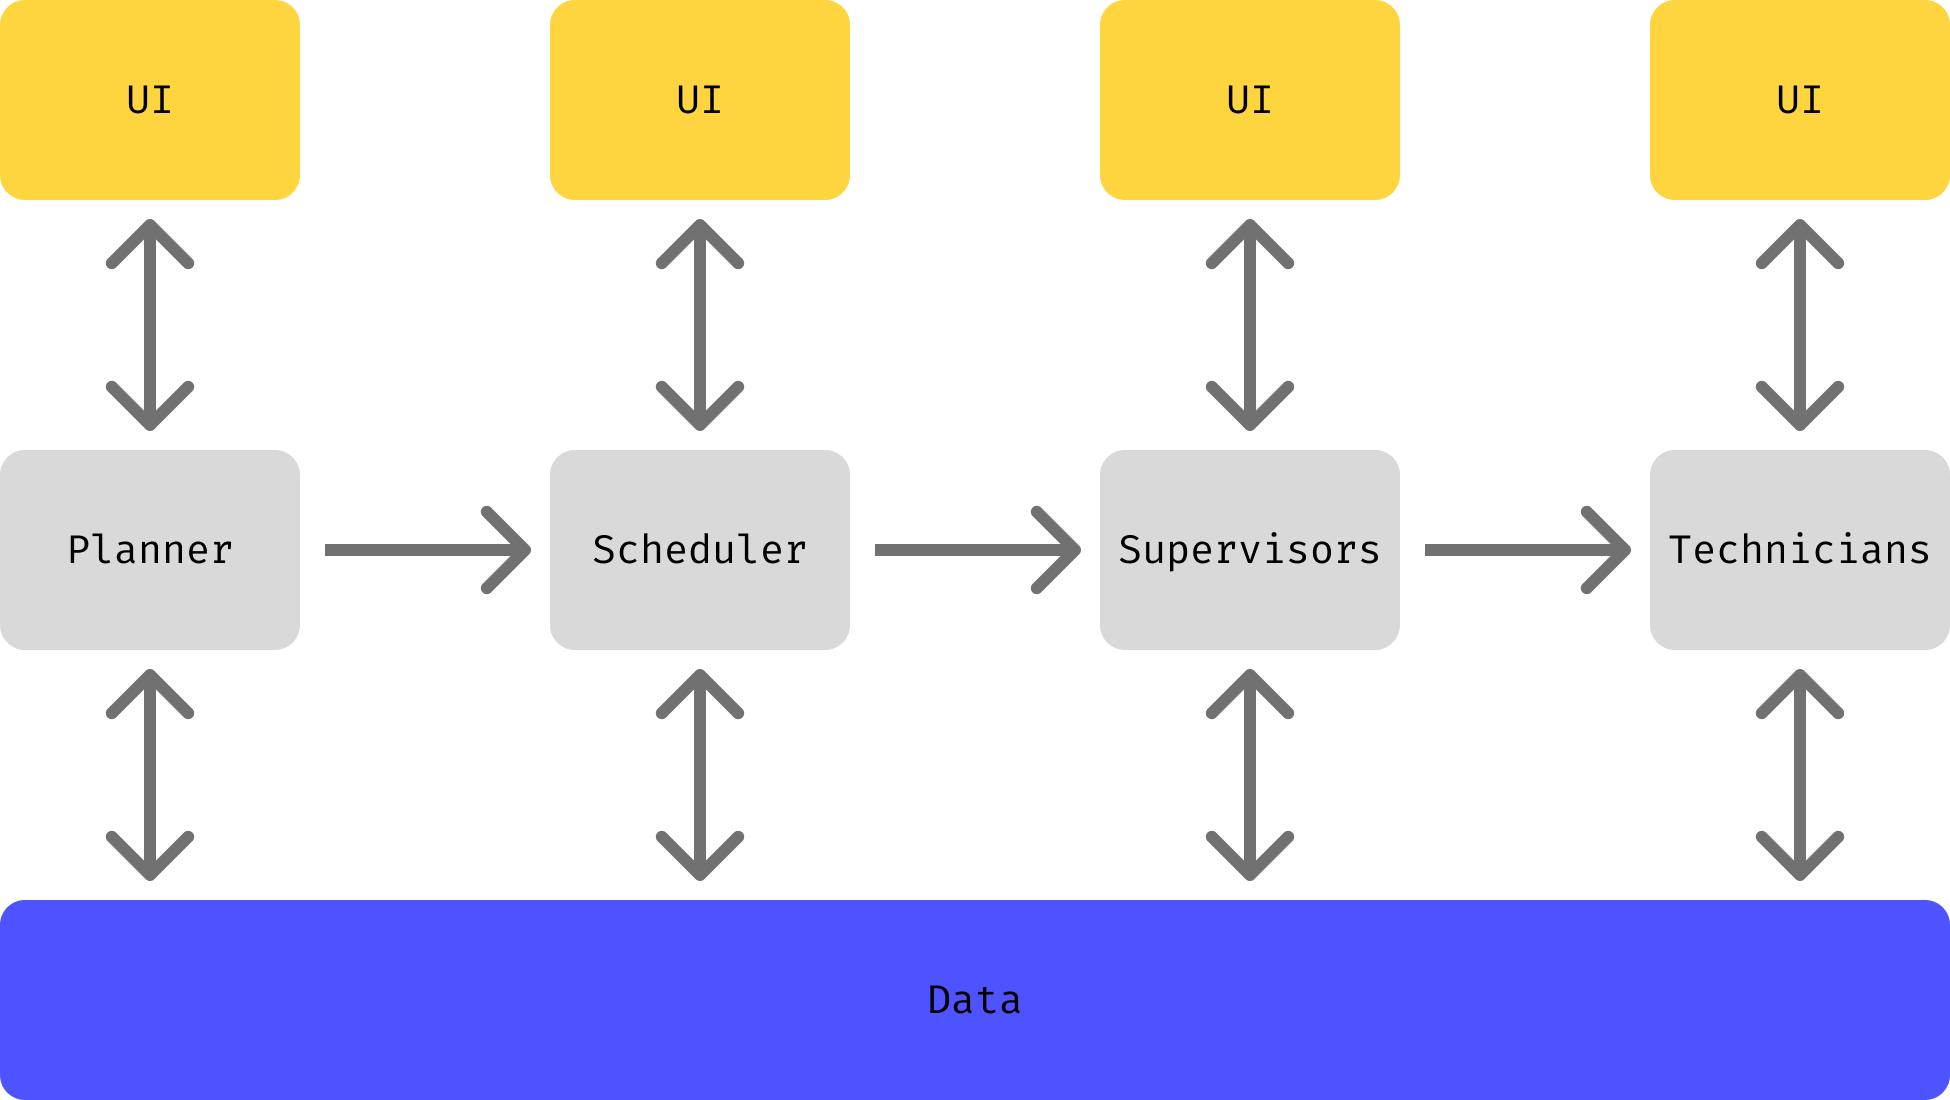
\includegraphics[width=1.0\textwidth]{figures/Scheduling Process Integrated.png}
\label{fig:integrated:maintenance-process}
\caption{Overview of the scheduling process when modelled as actors. When LNS is encapsulated 
is an actor it becomes possible to optimize parts of a large process individually instead of 
optimizing the scheduling problem globally from a single model inplementation.}
\end{figure}


\subsection{Continuous Optimization}
With actor-based metaheuristics it becomes simple to extend a metaheuristic to run
indefinitely with it being able to optimize based on the latest best 
available information. This may seem like a minor detail as you could argue that you should only ever optimize the schedule when there is 
an explicit need for it, but consider the case when you start adding more than two actor to a scheduling system, then there arises a need
to coordinate people in time as each will have to run their optimizer on after another.



\bibliography{refs}

\bibliographystyle{elsarticle-harv}
\end{document}

hello
\endinput
